\chapter{Japan's case study}
\renewcommand{\headrulewidth}{0pt}
\lhead[\thepage]{\leftmark}
\rhead[\leftmark]{\thepage}
\cfoot[]{}

\section{Introduction}
Nitrogen dioxide (NO2) is an important air pollutant that raises significant concerns due to its negative effects on human health \citep{hamra2015lung}. Additionally, it serves as a crucial precursor to tropospheric ozone (O3), along with volatile organic compounds (VOCs) \citep{akimoto2022rethinking}. Nitrogen oxides (NOx = NO + NO2), carbon monoxide (CO) and non-methane volatile organic compounds (NMVOCs) have an influence on the methane (CH4) lifetime by affecting the atmospheric mixing ratio of hydroxyl radicals (OH) \citep{akimoto2022rethinking}, which act as a primary sink for CH4 \citep{turner2019interpreting}. Both O3 and CH4 are short-lived climate pollutants (SLCPs) that contribute to positive radiative forcing, thereby intensifying global warming \citep{akimoto2022rethinking}. Moreover, owing to its short lifetime in the atmosphere and significant signal compared to carbon dioxide (CO2), NO2 possesses the potential to serve as an indicator for monitoring localized fossil fuel CO2 emissions \citep{miyazaki2023predictability}. \par

In 2020, the implementation of COVID-19 social distancing policies in multiple countries led to a significant decrease in human activities worldwide \citep{de2022overview}. While the general anticipation was for a reduction in NO2 emissions in many cities due to the decline in anthropogenic activities \citep{bauwens2020impact,barre2021estimating,cooper2022global}, the response of O3 and CH4 has been unexpected.\par

Increased levels of O3 have been observed in northern Europe, China, and South Africa as a consequence of the COVID-19 lockdown, according to sensitivity simulations conducted using the MIROC-CHASER global chemical transport model \citep{miyazaki2021global}. This rise in O3 can be attributed to the general reduction in NOx, which enhances O3 production by reducing NO titration in areas with high levels of NOx pollution or VOC-limited areas \citep{akimoto2022rethinking}. Furthermore, meteorological effects have played a significant role in the changes observed in O3 levels between 2020 and the reference year \citep{ordonez2020early,liu2021diverse}. Despite accounting for the influence of weather conditions, significant variations in O3 level estimates have been reported across studies, particularly in European countries \citep{ordonez2020early,grange2021covid}, and China \citep{liu2021diverse,shi2021abrupt}. The presence of sunlight is essential for the O3 generation in response to the decrease in NOx during the lockdown period. As a result, the lack of sunny conditions in specific urban areas at the time of the atmospheric response to NO2 reduction may have led to differing time delays before observable changes in O3 levels occurred \citep{grange2021covid} (Grange et al. 2021). \par

In 2020, during the COVID-19 pandemic, global CH4 emissions experienced a significant growth rate, which was contrary to the expected decrease in anthropogenic CH4 emissions due to the implementation of lockdown measures \citep{peng2022wetland}.  In 2020, anthropogenic CH4 emissions only slightly decreased compared to 2019, while wetland emissions rose sharply. This increase in wetland emissions was likely influenced by unusually warm and wet weather in the Northern Hemisphere \citep{peng2022wetland}, which could be connected to the impact of climate change \citep{zhang2023recent}. Apart from the variation in CH4 emission itself, it was found that the decrease in hydroxyl radical (OH) concentration due to changes in air pollutants like NOx, CO, and NMVOCs during the COVID-19 pandemic mainly accounted for approximately half (53 ± 10\%) of the observed global CH4 level growth in 2020 \citep{peng2022wetland}. A similar finding regarding the effect of NOx, CO, and NMVOCs emission changes on the 2020 methane levels is reported by \citep{stevenson2022covid}. However, other studies using Greenhouse gases Observing SATellite (GOSAT) observations indicated that most of observed increase in atmospheric CH4 during 2020 and 2021 can be attributed to increased CH4 emission itself \citep{qu2022attribution,feng2023methane}. Although CH4 has a long estimated lifetime of 8-10 years and has mostly been discussed at the global level, it is important to note that policies and approaches to address CH4 emissions may vary locally. \par

\begin{figure}[tbh!]
    \centering
    \begin{subfigure}{\textwidth}
      \centering
      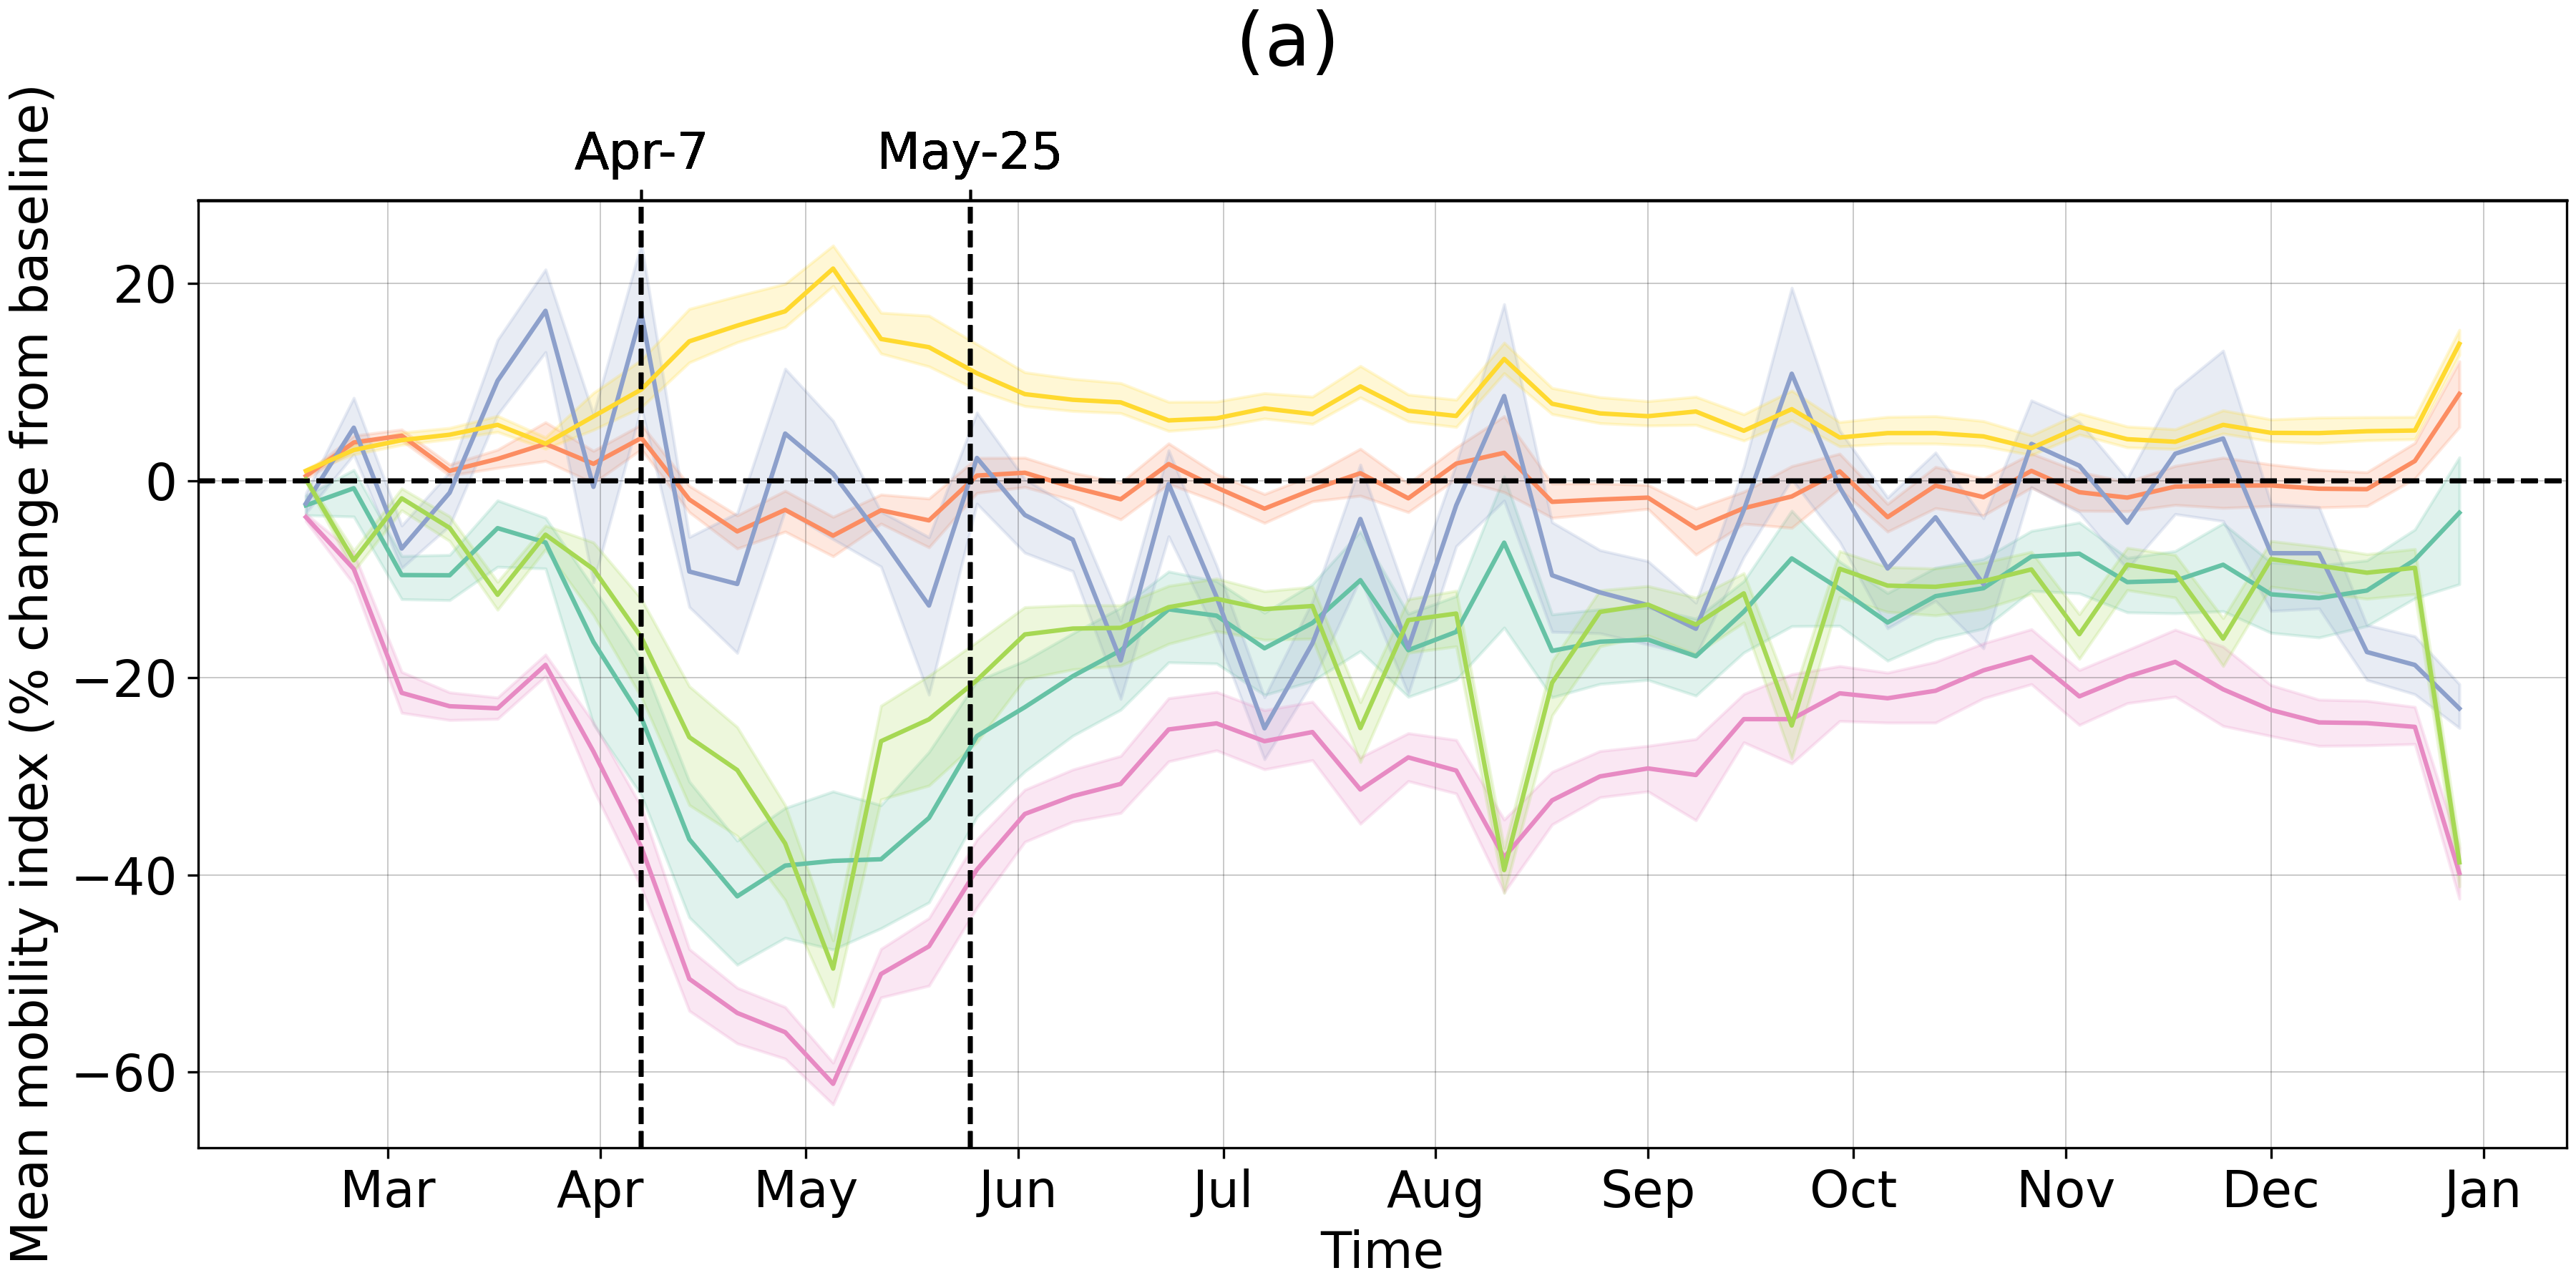
\includegraphics[width=\textwidth]{figs/chap4/fig1a_mobi_doy.png}
      \label{fig:chap4_fig1a}
    \end{subfigure}

    \begin{subfigure}{\textwidth}
      \centering
      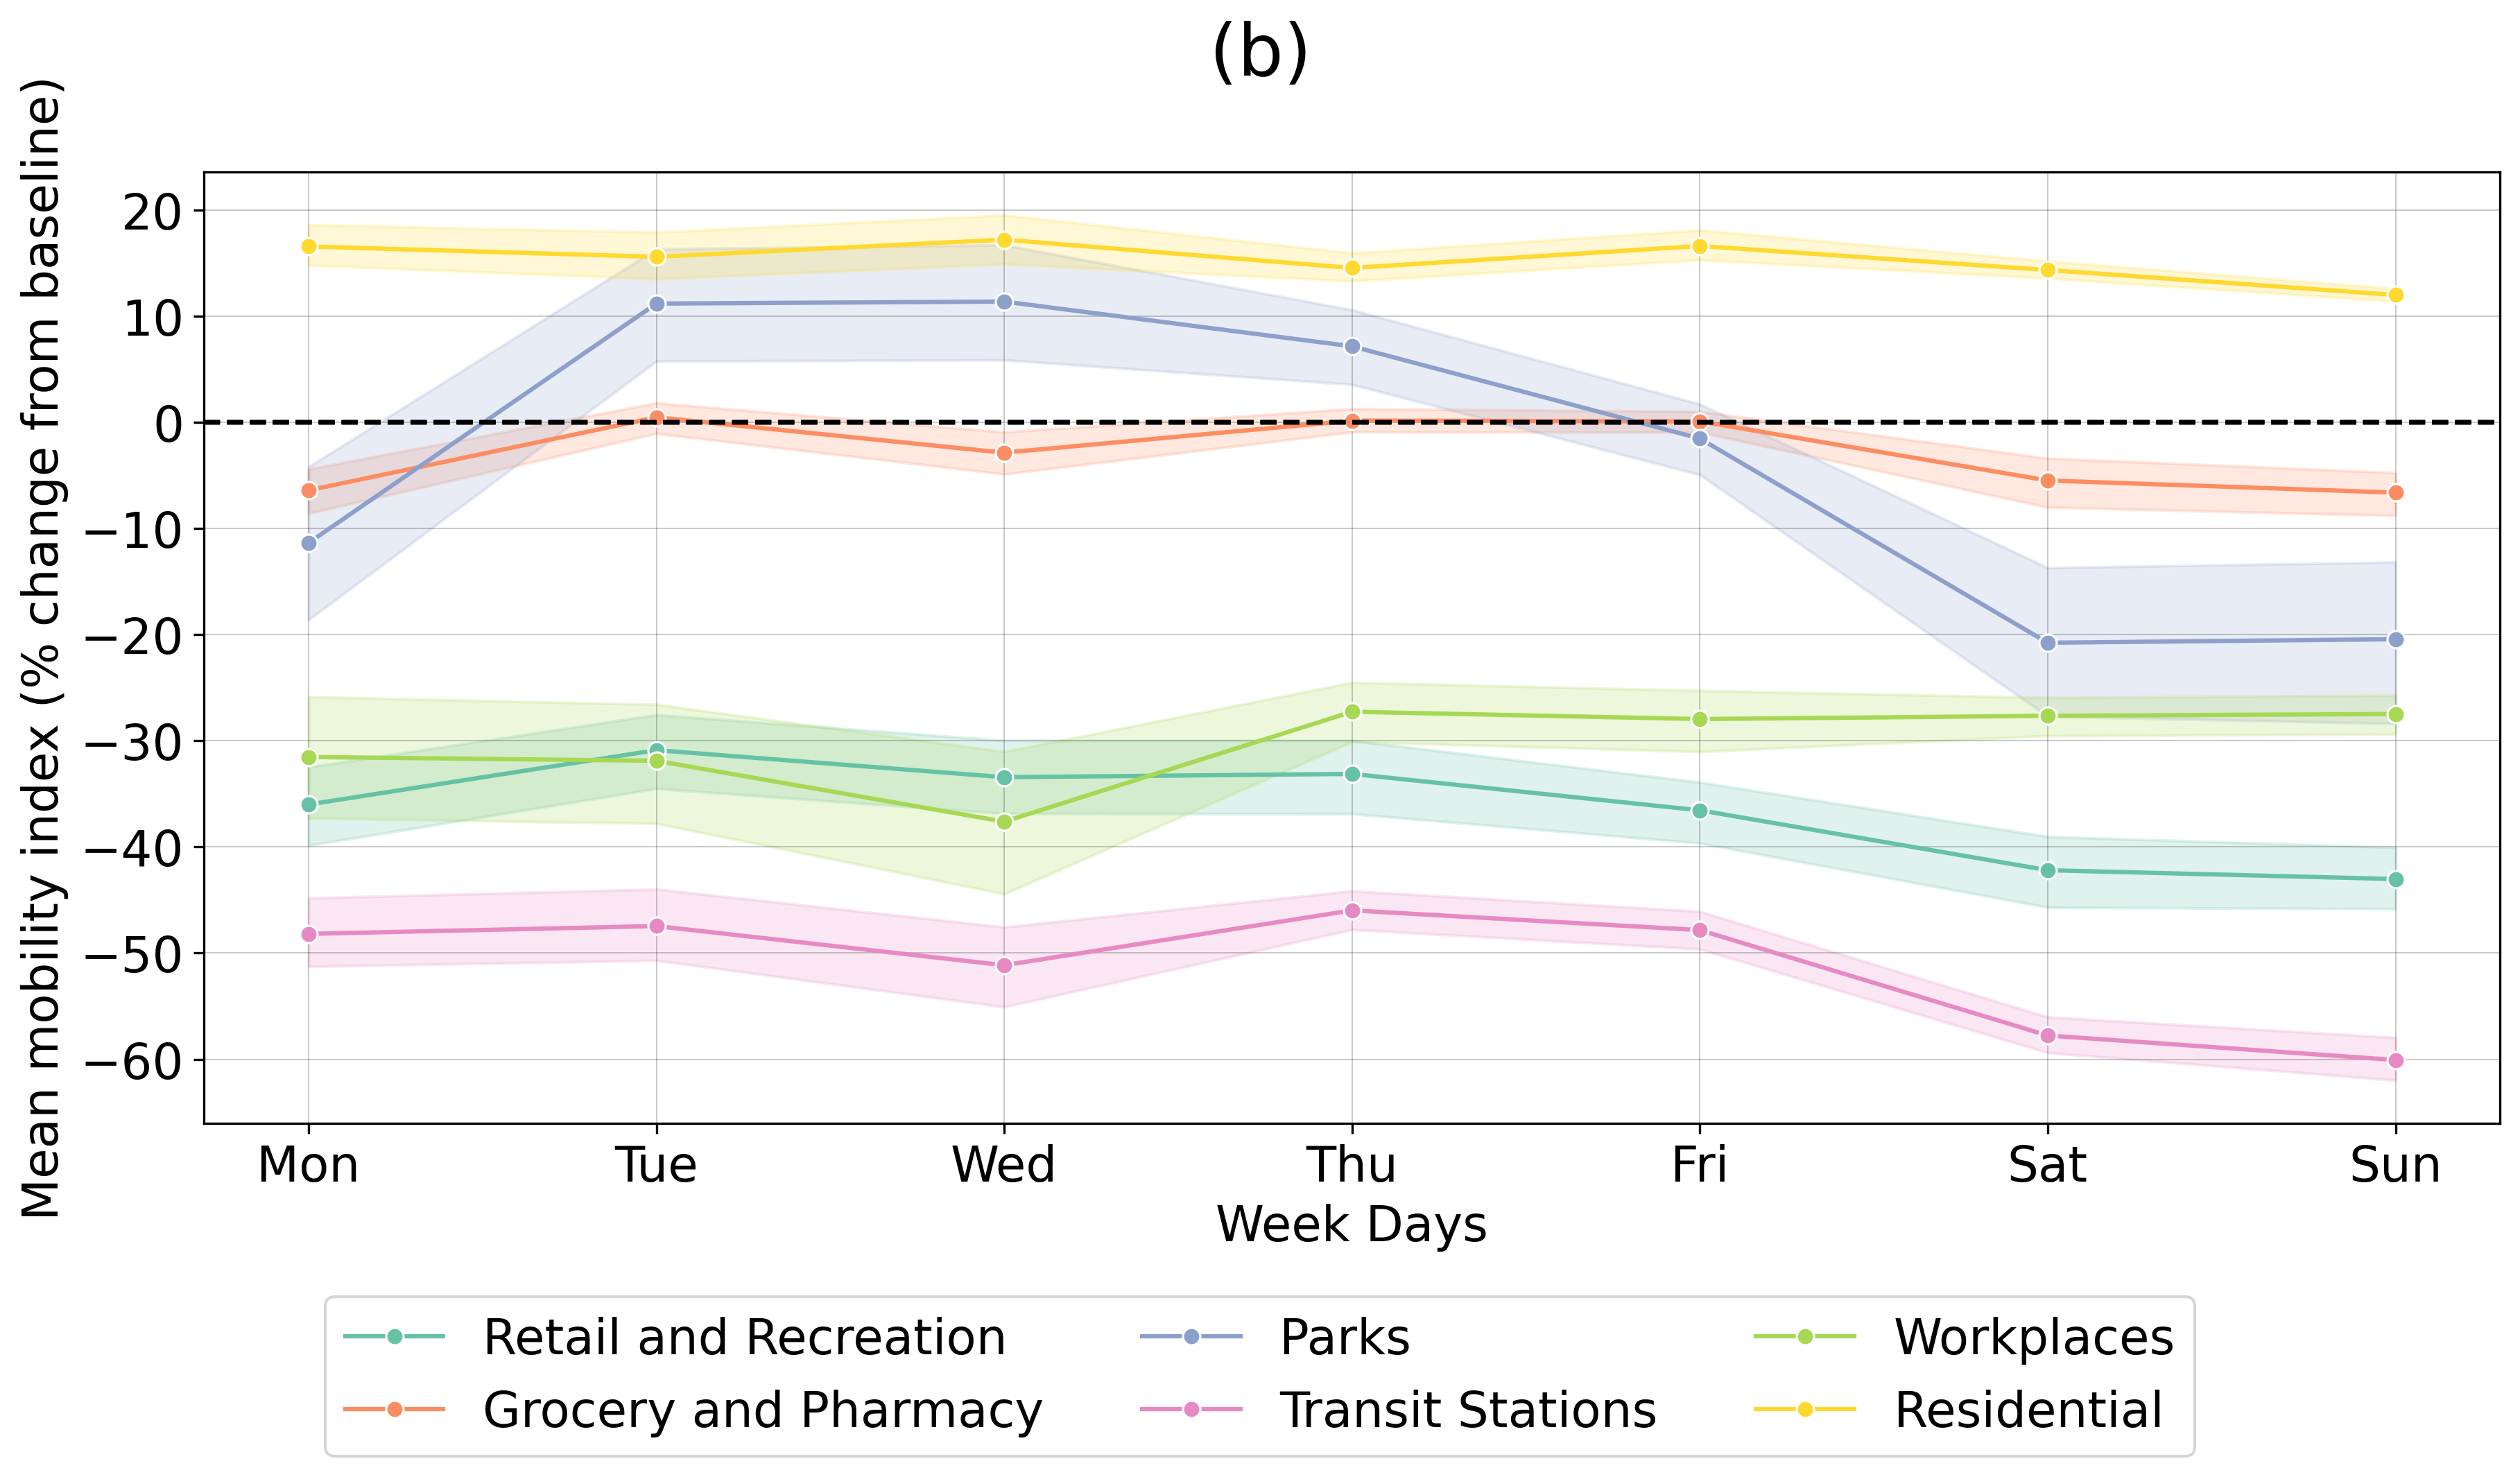
\includegraphics[width=\textwidth]{figs/chap4/fig1b_mobi_dow.png}
      \label{fig:chap4_fig1b}
    \end{subfigure}
    \caption[Mobility changes for 6 prefectures in Japan]{Mobility changes for 6 prefectures in Japan (Aichi, Fukuoka, Tokyo, Osaka, Kyoto, and Hyogo) in 2020 based on Google’s mobility indices for timeseries (a) and days of the week (b)}
    \label{fig:chap4_fig1}
\end{figure}

In 2020, Japan also experienced the impact of the COVID-19 pandemic, and in response to prevent the virus's spread, a state of emergency was declared from April 7 to May 25. This measure resulted in the suspension of various economic activities and imposed restrictions on people's mobility. As a consequence, there was a significant decline (Figure 1) in a unique weekend movement trend \citep{damiani2022peculiar}. \par

Although the primary aim of the lockdown was not specifically to address air pollution and greenhouse gas emissions, the implementation of these measures offers valuable insights for atmospheric modelling. It provides practical knowledge and first-hand experience to develop more efficient strategies for mitigating air pollution and reducing greenhouse gas emissions in the future \citep{grange2021covid}. It is important to note that the changes in air pollutants during this period varied across regions and were strongly influenced by meteorological conditions. Performing a regional analysis of these changes can provide evidence to support the formulation of appropriate regional policies in the future. In this study, our objective is to evaluate the impact of changes in anthropogenic activities during the COVID-19 pandemic (from April 7 to December 31) on NO2, O3, CO and CH4 in metropolitan areas (MAs) of Japan in 2020, which have not been thoroughly investigated in previous studies. \par

In the first phase (Section \ref{chap4_data}), we gathered data from ground observations, satellite sources, and biogeochemical model simulations. Subsequently, we constructed a weather normalization model under business-as-usual (BAU) conditions utilizing machine learning techniques, incorporating meteorological, spatial, and temporal predictors (Section \ref{chap4_method}). We investigated variations in air pollution levels by analysing the BAU predictions alongside additional data in Section \ref{chap4_result}. Lastly, we provided discussions in Section \ref{chap4_disscussion}, while in Section \ref{chap4_conclusion}, we present our study's findings, conclusions, and recommendations for future policy considerations.\par

\section{Data} \label{chap4_data}
\subsection{Study area}
Prior research primarily focused on assessing the impact of pandemic lockdown measures on air quality within the Greater Tokyo Area, being the most densely populated metropolitan area globally \citep{damiani2022peculiar,zoran2023peculiar}. Nevertheless, there's a notable absence of similar analyses for other MAs. Our study covers 14 MAs in Japan, extending from Sapporo in the north to Kagoshima in the south, as depicted in Figure 2. We focus on these metropolitan areas due to their housing of Japan's highly populated and vibrant cities, which are intricately connected with human activities and air pollution in Japan.\par
\begin{figure}[p]
    \centering
    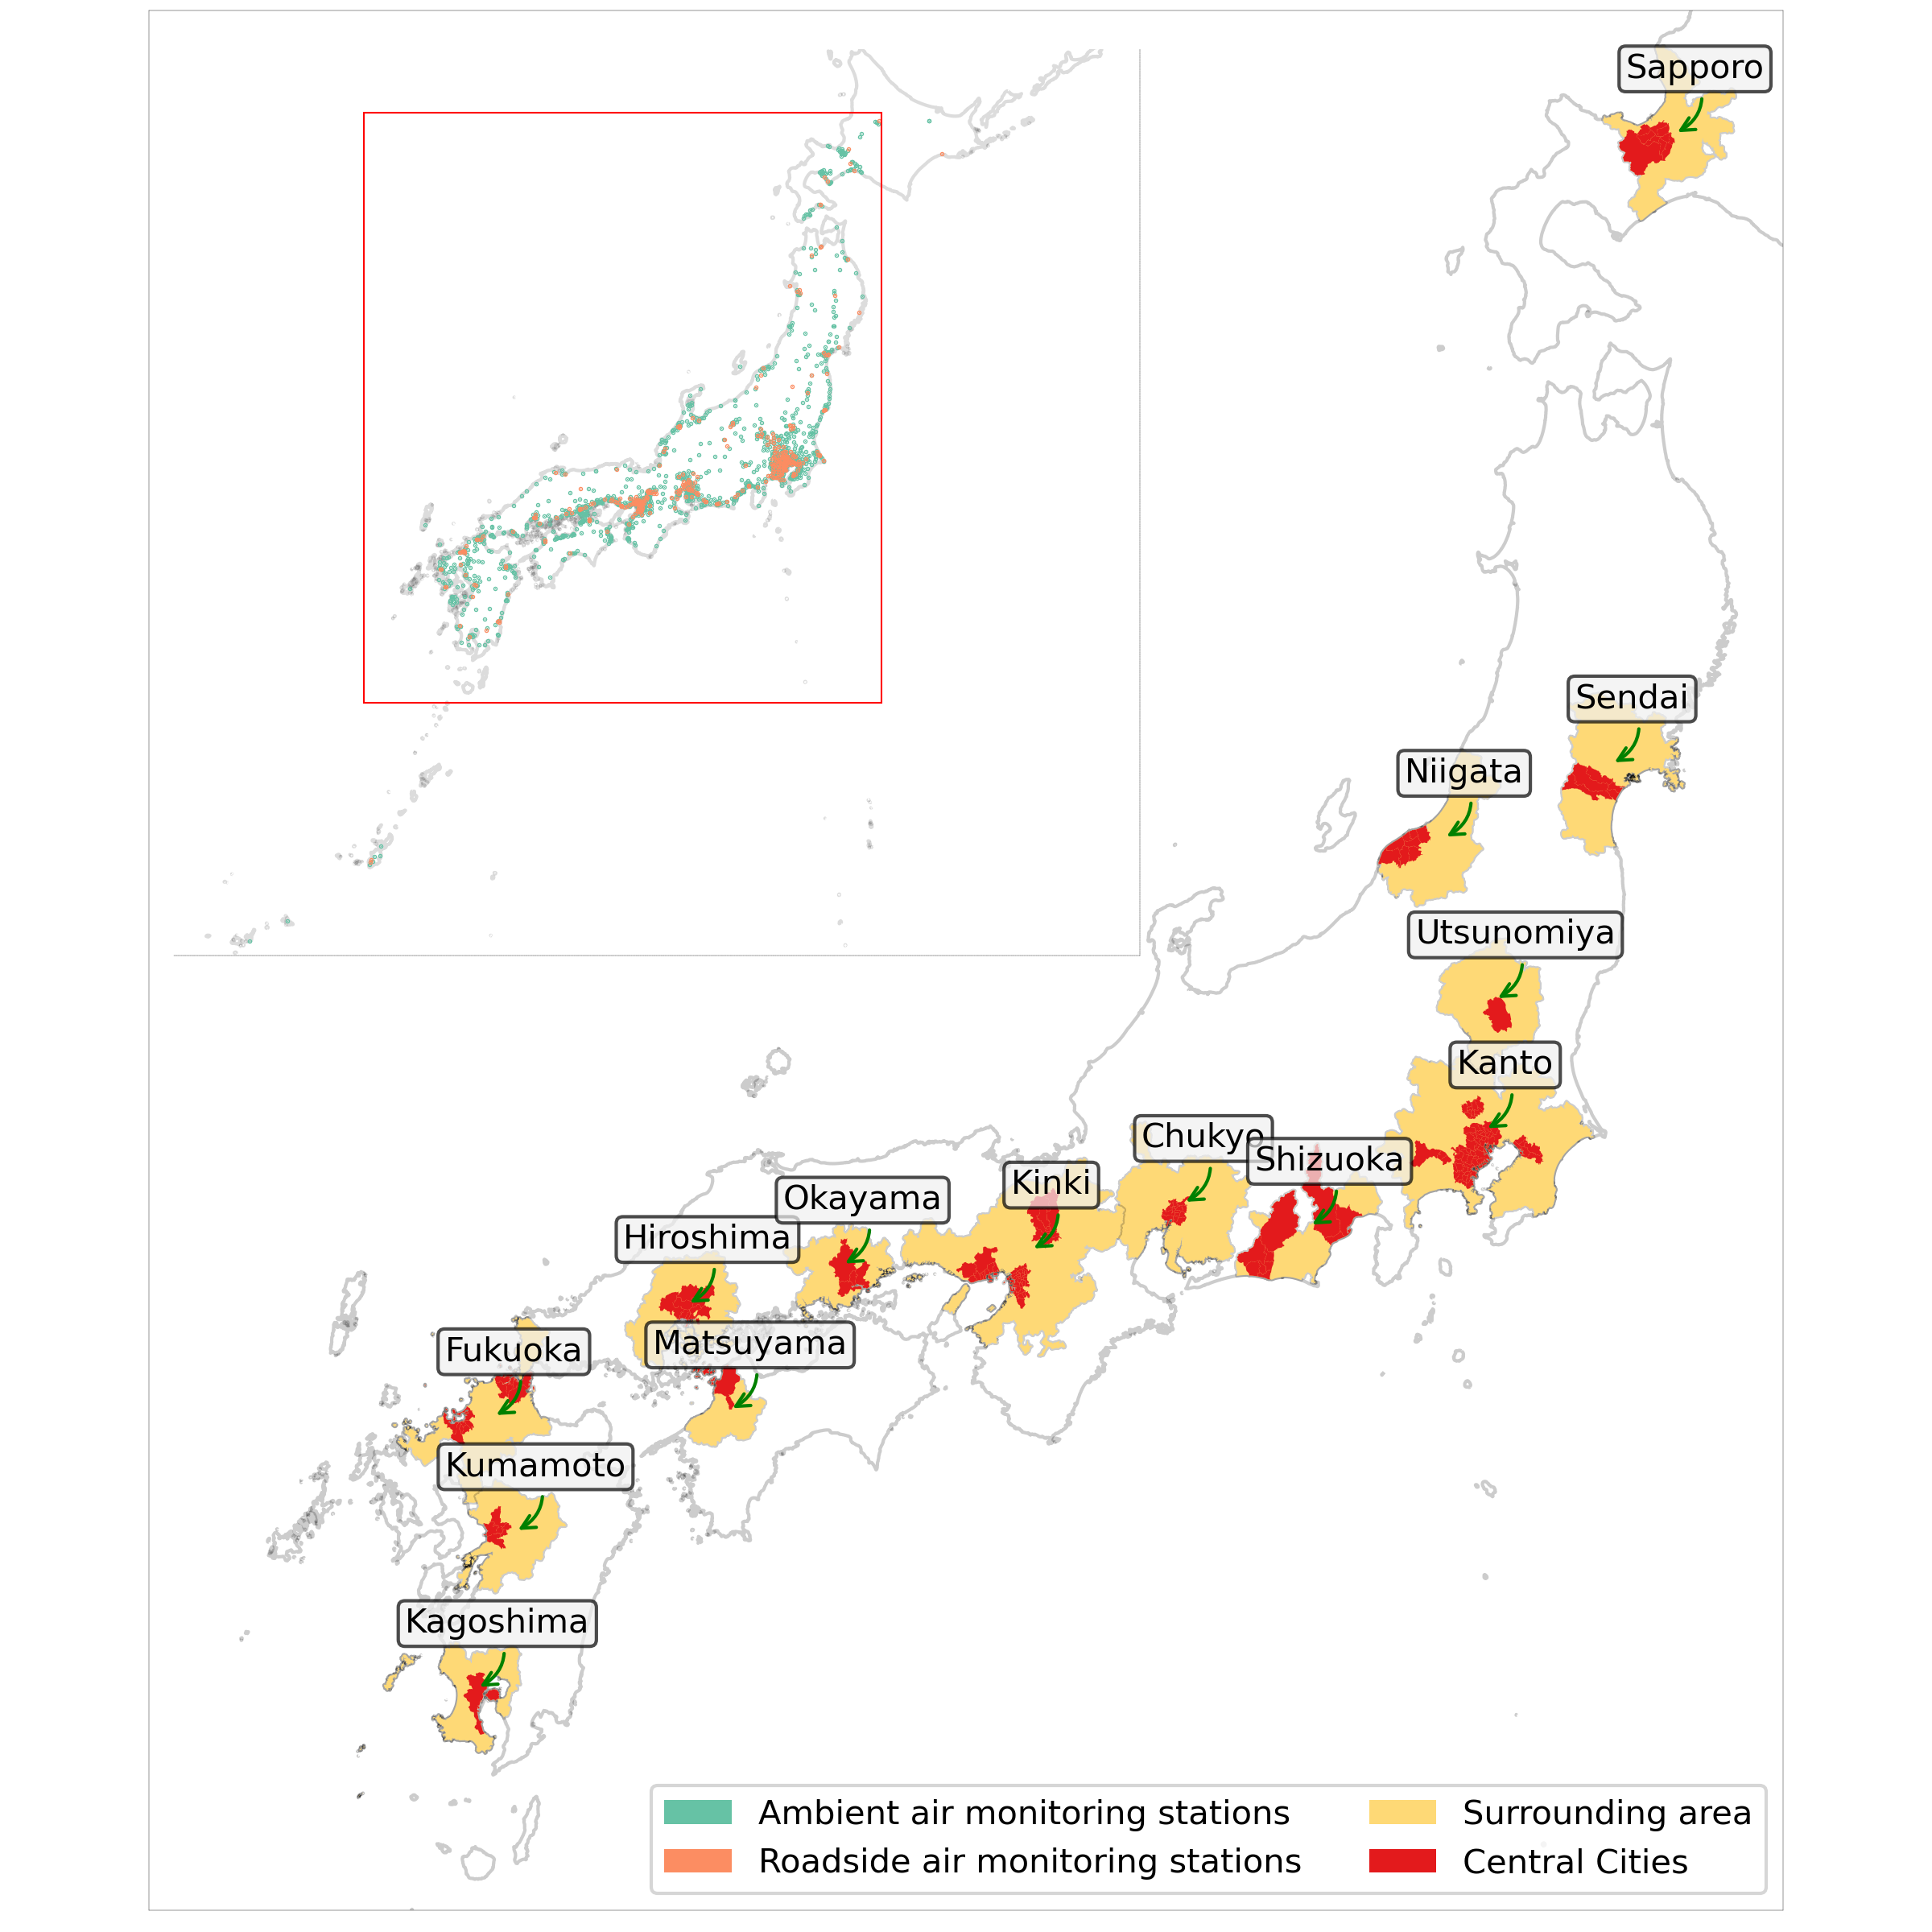
\includegraphics[width=\textwidth]{figs/chap4/fig2.png}
    \caption[Study area]{The locations of 14 metropolitans’ areas and the distribution of ground observations for air quality monitoring in Japan}
    \label{fig:chap4_fig2}
\end{figure}
\subsection{Ground observation}
To acquire air quality data, we gathered ground observations for NO2, O3, CO, and CH4 from the air quality monitoring data archive published by the National Institute for Environmental Studies (NIES). These observations spanned a ten-year period from 2010 to 2020 and were collected from 1,180 stations for NO2, 835 stations for O3, 383 stations for CH4, and 237 stations for CO. The study utilized two types of stations: roadside air monitoring stations (RsAMS), which are placed in areas prone to air pollution from vehicle exhaust caused by traffic congestion, like intersections, roads, and near road edges, and ambient air monitoring stations (AAMS), which are established to assess air pollution in general living spaces such as residential areas. These station types have been categorized by NIES, and the data can be readily acquired from the original downloadable dataset. \par
Apart from air quality data, we incorporated ground observations of meteorological data from Japan Meteorological Agency (JMA) as input features for the BAU models used in the study. Specifically, we obtained daily records from 52 weather stations located within the same 14 MAs. At each weather station, we gathered temperature, wind direction and speed, local atmospheric pressure, and relative humidity, as suggested by \citep{grange2021covid}. The corresponding meteorological parameters were extracted from the nearest weather observation site for each air quality station.\par

\subsection{ERA5 reanalysis dataset}
Alongside the weather data collected from the ground stations in the NIES database, for the features of the BAU models, we incorporated additional daily data pertaining to boundary layer height, total cloud cover, downward solar radiation (SR), and total precipitation, as recommended by \citep{shi2021abrupt}. This supplementary information was sourced from the ERA5 reanalysis dataset (ERA5 hourly data on single levels from 1940 to the present) obtained from the Climate Data Store of the Copernicus Climate Change Service. Additionlly, the ERA5 2m temperature variable (T2M) and SR will be utilized to assess the variation of sunny conditions during both the lockdown and post-lockdown periods within the study area. The original ERA5 data possesses a spatial resolution of 0.25$^{\circ}$ $\times$ 0.25$^{\circ}$ .\par
\subsection{Sentinel 5P TROPOMI}
In this study, we utilized the Sentinel 5P (S5P) Tropospheric Monitoring Instrument (TROPOMI) data to evaluate the tropospheric formaldehyde-to-NO2 ratio (FNR) specifically for the year 2020. This ratio serves as a key indicator for the sensitivity of tropospheric ozone production. The tropospheric NO2 and formaldehyde (HCHO – as a proxy for NMVOCs) data was obtained from the S5P L3 product \enquote{OFFL\slash L3\_NO2} (based on processor version 1.2.x and 1.3.x) and \enquote{OFFL\slash L3\_HCHO} (based on processor version 1.1.x) collections from Google Earth Engine, respectively. To generate the comprehensive L3 S5P product, each operational level (L2) product underwent preprocessing and mosaicking using the harpconvert tool. The low-quality pixels was filtered out in L3 NO2 product by excluding those with AQ (Air Quality) values below 75\% for the band \enquote{tropospheric\_NO2\_column\_number\_density}. The resulting data, ready for download, is available with a spatial resolution of about 1$\times$1 km2.
\subsection{Biogeochemical modelled CH4 budget}
In our assessment of CH4 emission variations, with a specific focus on emissions from natural sources such as wetlands, we utilized CH4 budget data obtained from the Vegetation Integrative SImulator for Trace gases (VISIT) \citep{ito2019methane}. VISIT is a biogeochemical model that takes into account historical land use and climatic conditions to estimate CH4 emissions \citep{ito2019methane}. The CH4 budgets generated by the VISIT model are now available and accessible through the Global Environmental Database provided by NIES, Japan \citep{ito2019methane}. We utilized the global data versions \enquote{Ver.2021.1\_CH4Wetl\_Cao} \citep{ito2021cao}, and \enquote{Ver.2021.1\_CH4Wetl\_WH} \citep{ito2021wh}, which incorporate Cao scheme \citep{cao1996global}, and Walter and Heimann scheme (WH scheme) \citep{walter2000process}, to estimate CH4 emission for each MA, which offers CH4 emission information at a spatial resolution of 0.5$^{\circ}$ $\times$ 0.5$^{\circ}$. \par
\section{Method} \label{chap4_method}
\subsection{Business-as-usual (BAU) modelling}
To accurately quantify the actual change in the levels of the four pollutants, we developed a weather normalization model under BAU conditions using machine learning. This model was specifically designed to simulate pollutant levels without the influence of COVID-19 restriction measures, using meteorological, spatial, and temporal features as inputs. The meteorological predictors utilized in our model include ground observation data such as temperature, wind direction and speed, local atmospheric pressure, and relative humidity. Additionally, we incorporated data from the ERA5 reanalysis dataset, which comprises boundary layer height, total cloud cover, downward solar radiation, and total precipitation. Temporal predictors included the Julian date (the number of days since January 1) and the day of the week. Furthermore, latitude and longitude coordinates of each station were utilized as spatial predictors. To develop the weather normalization models for each pollutant at both AAMS and RsAMS, we utilized data from the years 2016 to 2019, which offers a comprehensive timeframe to account for the diverse air pollution concentration fluctuations experienced across various meteorological conditions. Extending the period, such as from 2010 to 2019, would not accurately represent recent air quality trends due to the impact of past air pollution reduction policies. Conversely, a shorter timeframe, such as the pre-lockdown period months would not adequately capture the full range of meteorological variations. Overall, four separate weather normalization models were developed for each pollutant (NO2, O3, CO, and CH4), taking into account the specific station type (RsAMS and AAMS). \par

\begin{figure}[tbh!]
    \centering
    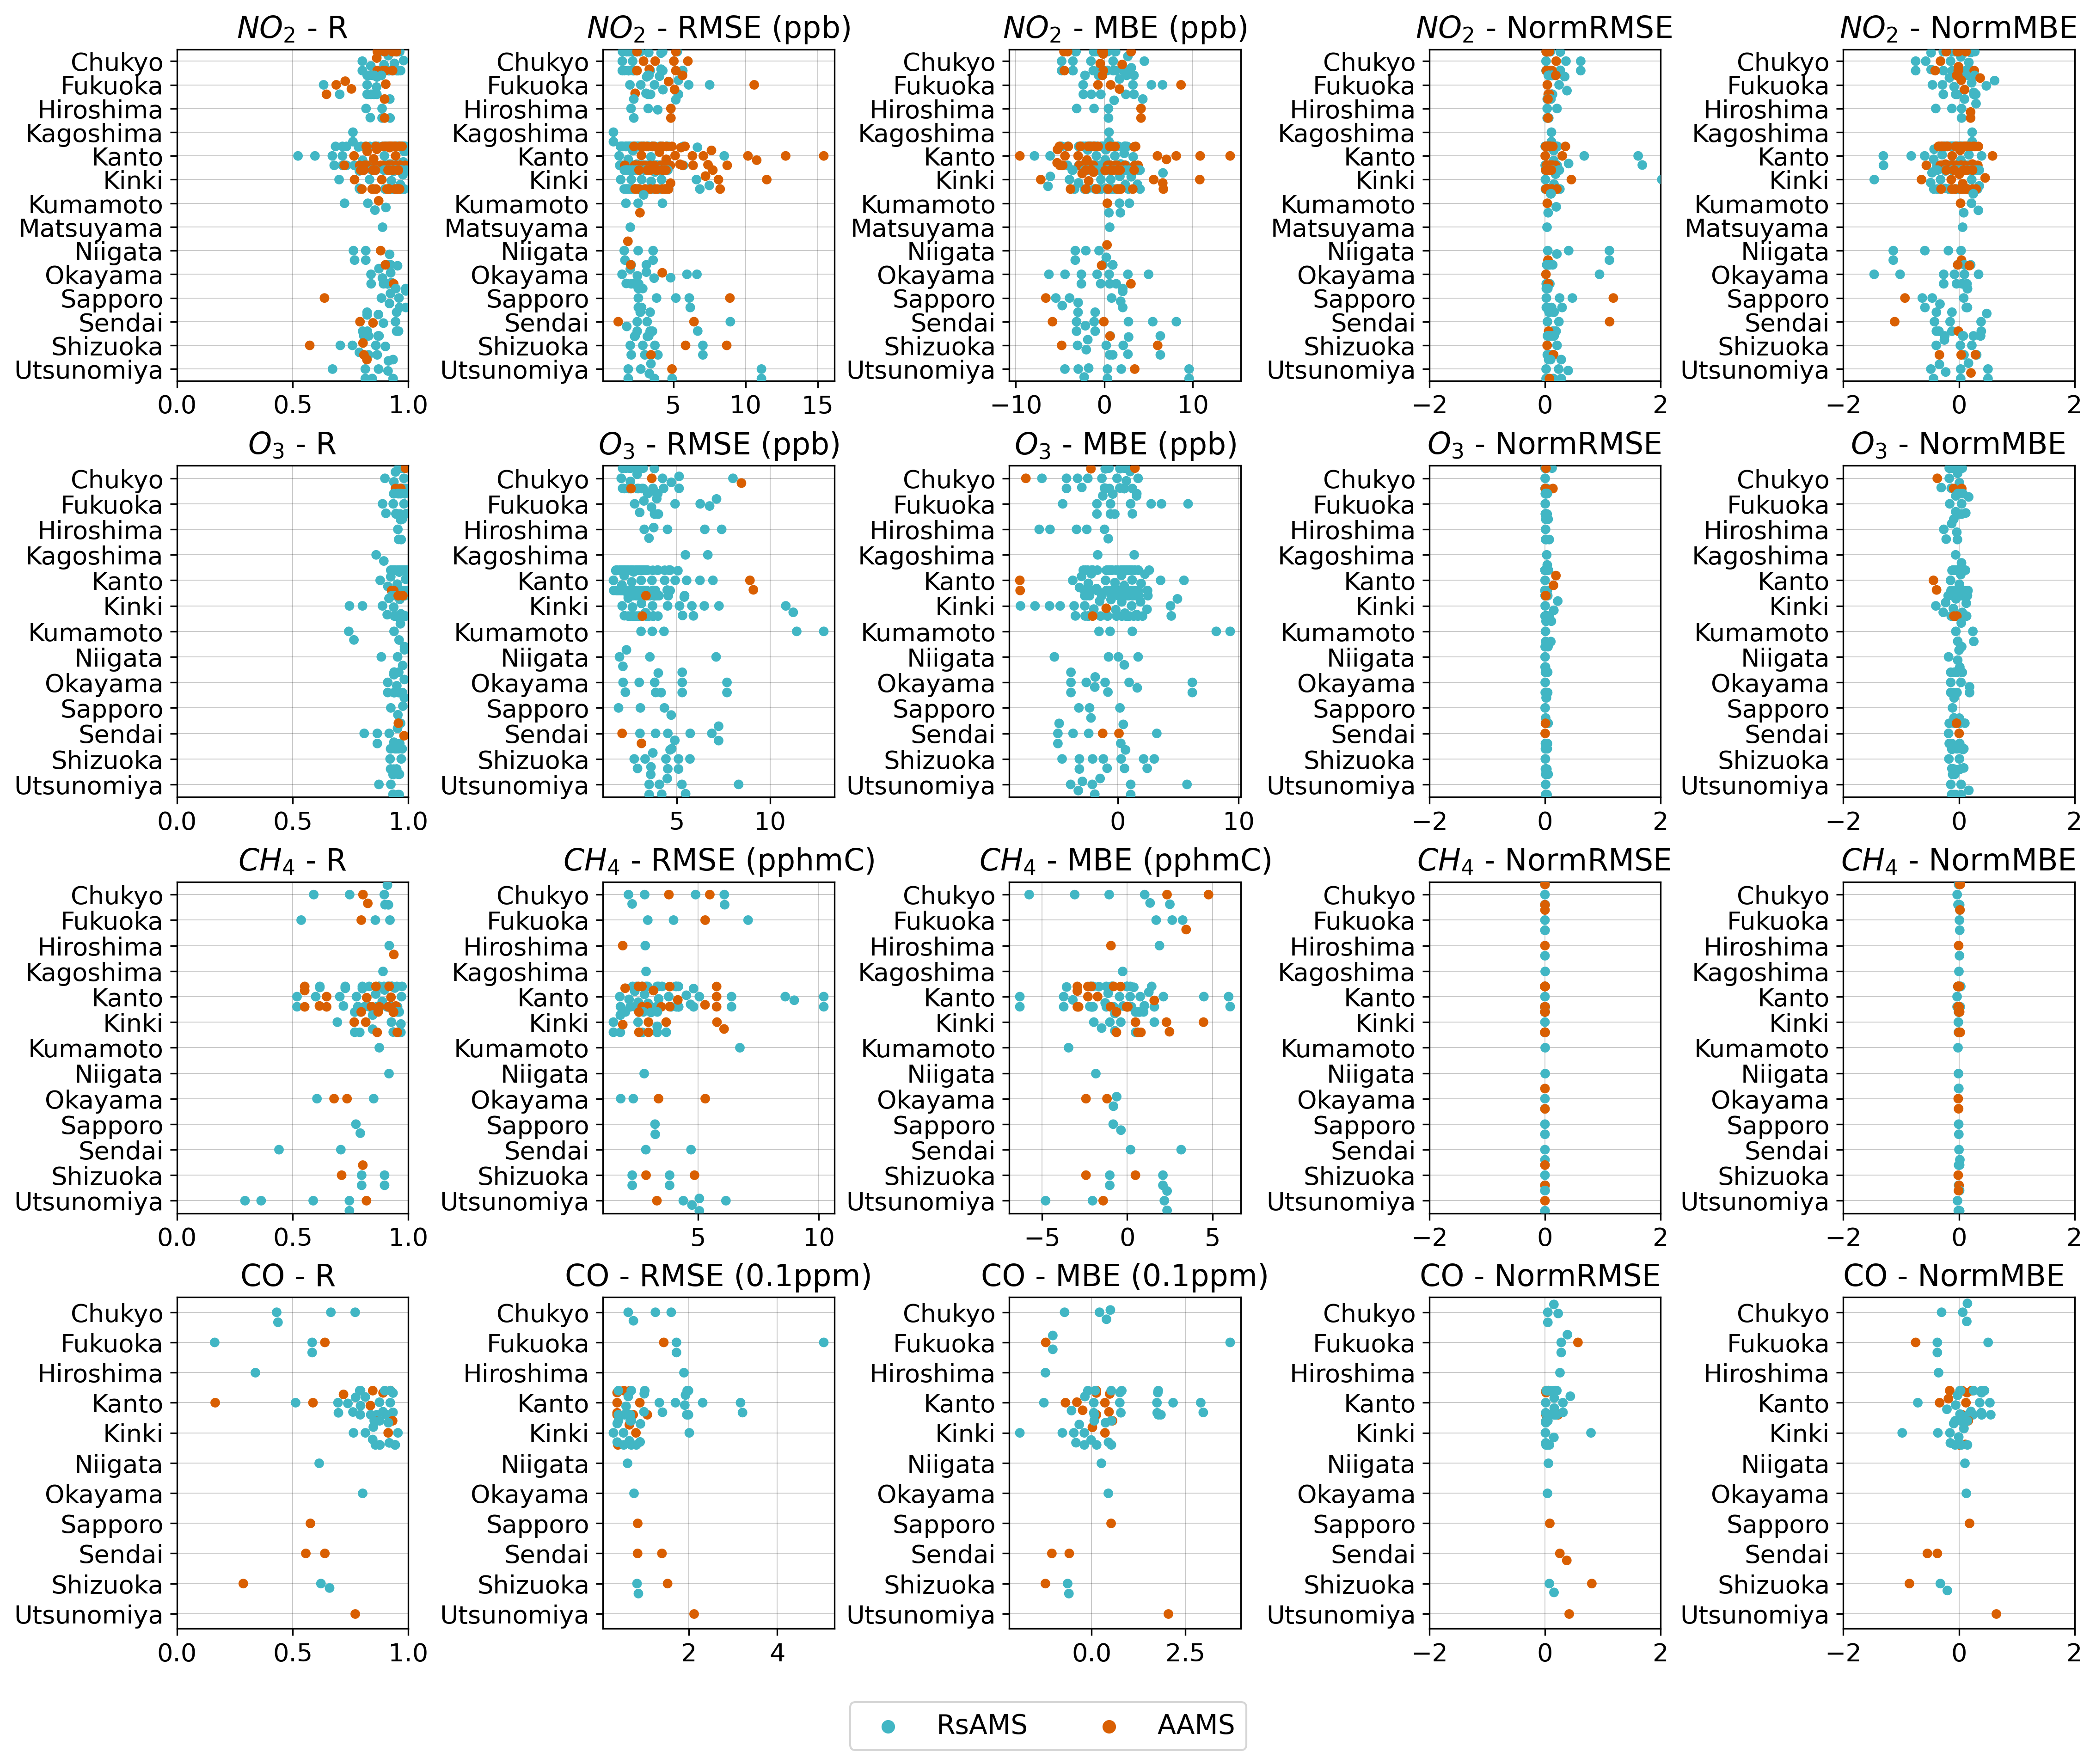
\includegraphics[width=\textwidth]{figs/chap4/fig3.png}
    \caption[Model performance evaluation]{The details score of each station on the test set. For each station on the test set, we calculated the following scores and display it in this figure: Pearson correlation coefficient (R), root mean square error (RMSE), normalized root mean square error (NormRMSE) and mean bias error (MBE), normalized mean bias error (NormMBE)}
    \label{fig:chap4_fig3}
\end{figure}

\begin{table}[!ht]
    \centering
    \caption[Model performance evaluation]{The performance of BAU model on the test set (30\% station data) with the following metrics: Pearson correlation coefficient (R), root mean square error (RMSE), normalized root mean square error (NormRMSE) and mean bias error (MBE), normalized mean bias error (NormMBE). For the normalized MBE and RMSE, we normalize values for each station and then compute the mean}
    \begin{tabular}{c c c c c c c}
        \hline
        Pollutants & Station type & R & RMSE & NormRMSE & MBE & NormMBE \\ \hline
        \multirow{2}{*}{NO2}    & AAMS & 0.89 & 3.13 & 0.15 & -0.12 & -0.07  \\
            & RsAMS & 0.88 & 4.84 & 0.10 & 0.30 & -0.03  \\ \hline
        \multirow{2}{*}{O3}    & AAMS & 0.96 & 3.75 & 0.02 & -0.37 & -0.02  \\
            & RsAMS & 0.96 & 4.92 & 0.06 & -3.18 & -0.16  \\ \hline
        \multirow{2}{*}{CO}    & AAMS & 0.73 & 0.84 & 0.17 & 0.00 & -0.07  \\
            & RsAMS & 0.77 & 1.23 & 0.13 & 0.39 & 0.04  \\ \hline
        \multirow{2}{*}{CH4}    & AAMS & 0.82 & 3.75 & 0.00 & -0.29 & 0.00  \\
            & RsAMS & 0.80 & 3.82 & 0.00 & -0.26 & 0.00  \\ \hline
    \end{tabular}
    \label{tab:chap4_tab1}
\end{table}

We employed the LightGBM machine learning model \citep{ke2017lightgbm}, a gradient boosting decision tree algorithm, to construct the BAU model using the aforementioned predictors. To fine-tune the model's hyperparameters, we utilized Fast and Lightweight AutoML Library (FLAML) \citep{wang2021flaml}, a lightweight library specifically designed for accurately identifying optimal hyperparameters for models. During the training process, we utilized 70\% of the station data within each metropolitan area (MA), while the remaining 30\% was reserved for validating the model's performance. Both the training and test data sets were randomly selected for each MA, ensuring unbiased representation across the dataset.\par

In order to evaluate the performance of the BAU model we utilized the following metrics mean bias error (MBE), normalized mean bias error (NormMBE), root mean square error (RMSE), normalized root mean square error (NormRMSE) and Pearson correlation coefficient (R) as suggested by \citep{grange2021covid}. The detailed results are presented in Figure 3 for each pollutant and station, average scores are shown in Table 1. In general, the model demonstrated strong performance with high R values (mostly R > 0.8) and low MBE and RMSE scores when applied to the test set for NO2, O3, and CH4. Regarding CO, the model achieved a satisfactory R value (R > 0.73).\par

\subsection{Experiments design}
Our aim is to assess the alterations in NO2 levels within 14 MAs during both the lockdown and post-lockdown periods in 2020. We also intend to explore how changes in NO2 may influence the shifts in O3 and CH4 levels in each of these timeframes. Notably, we were encouraged to undertake this investigation by an observation of an unusual O3 response to NO2 reduction in the Greater Tokyo Area \citep{damiani2022peculiar}, prompting me to study the response of O3 and CH4 in all 14 MAs across Japan. \par
We conducted three experiments to assess the impact of NO2 changes on O3 and CH4 levels. In the first experiment, we focused solely on quantifying the change in NO2 levels using the time series observations and "OBS-BAU" estimate which involved subtracting the BAU prediction from the observed data (OBS). In the second experiment, we expanded the analysis to include O3, incorporating additional variables  from the ERA5 (temperature – T2M and SR) and S5P datasets (FNR and HCHO). The last experiment included CH4, incorporating the "OBS-BAU" estimate for CH4 and NO2, as well as the "OBS-BAU" estimate for CO and simulated CH4 emissions from wetlands using the VISIT model. \par
For the experiments, we selected April 7 to May 25 as the lockdown period, August 1\textminus31 as the post-lockdown period for O3 analysis, and June 1 to December 31 for CH4 analysis. We selected these timeframes to better understand how the four air pollutants changed in response to the unforeseen COVID-19 lockdown measures and the period after the lockdown. \par

\section{Results} \label{chap4_result}
\subsection{NO2 level changes}
We initially examined the monthly trend of observed NO2 concentration levels across 1,180 stations in the 14 MAs from 2010 to 2019, and we compared these trends with the NO2 levels observed during the lockdown in 2020 as depicted in Figure 4a. The results indicate that the actual reduction in NO2 levels during the lockdown in 2020 is lower than the trend observed during 2010-2019, specifically 2.7 ppb for RsAMS and 2.2 ppb for AAMS. This implies that the NO2 levels observed during the lockdown were equivalent to those in 2023 for RsAMS and 2025 for AAMS, based on the trend observed during 2010-2019. \par

Prior studies have indicated the importance of considering meteorological factors when evaluating the effects of intervention measures \citep{ordonez2020early,grange2021covid,shi2021abrupt}. In order to accurately assess the impact of the lockdown while isolating the effects of weather conditions, we computed the "OBS-BAU" estimates for all MAs as depicted in Figure 4b. Additionally, Figure 4c presents the complete time series of NO2 levels in 2020 (OBS), the expected levels without the lockdown (BAU), and the average data from 2016-2019 for four MAs (Kanto, Kinki, Chukyo, Fukuoka). We only show the figures for four MAs to avoid overwhelming complexity and to provide a more manageable representation of the figures. \par

\begin{figure}[tbh!]
    \centering
    \begin{subfigure}{.5\textwidth}
      \centering
      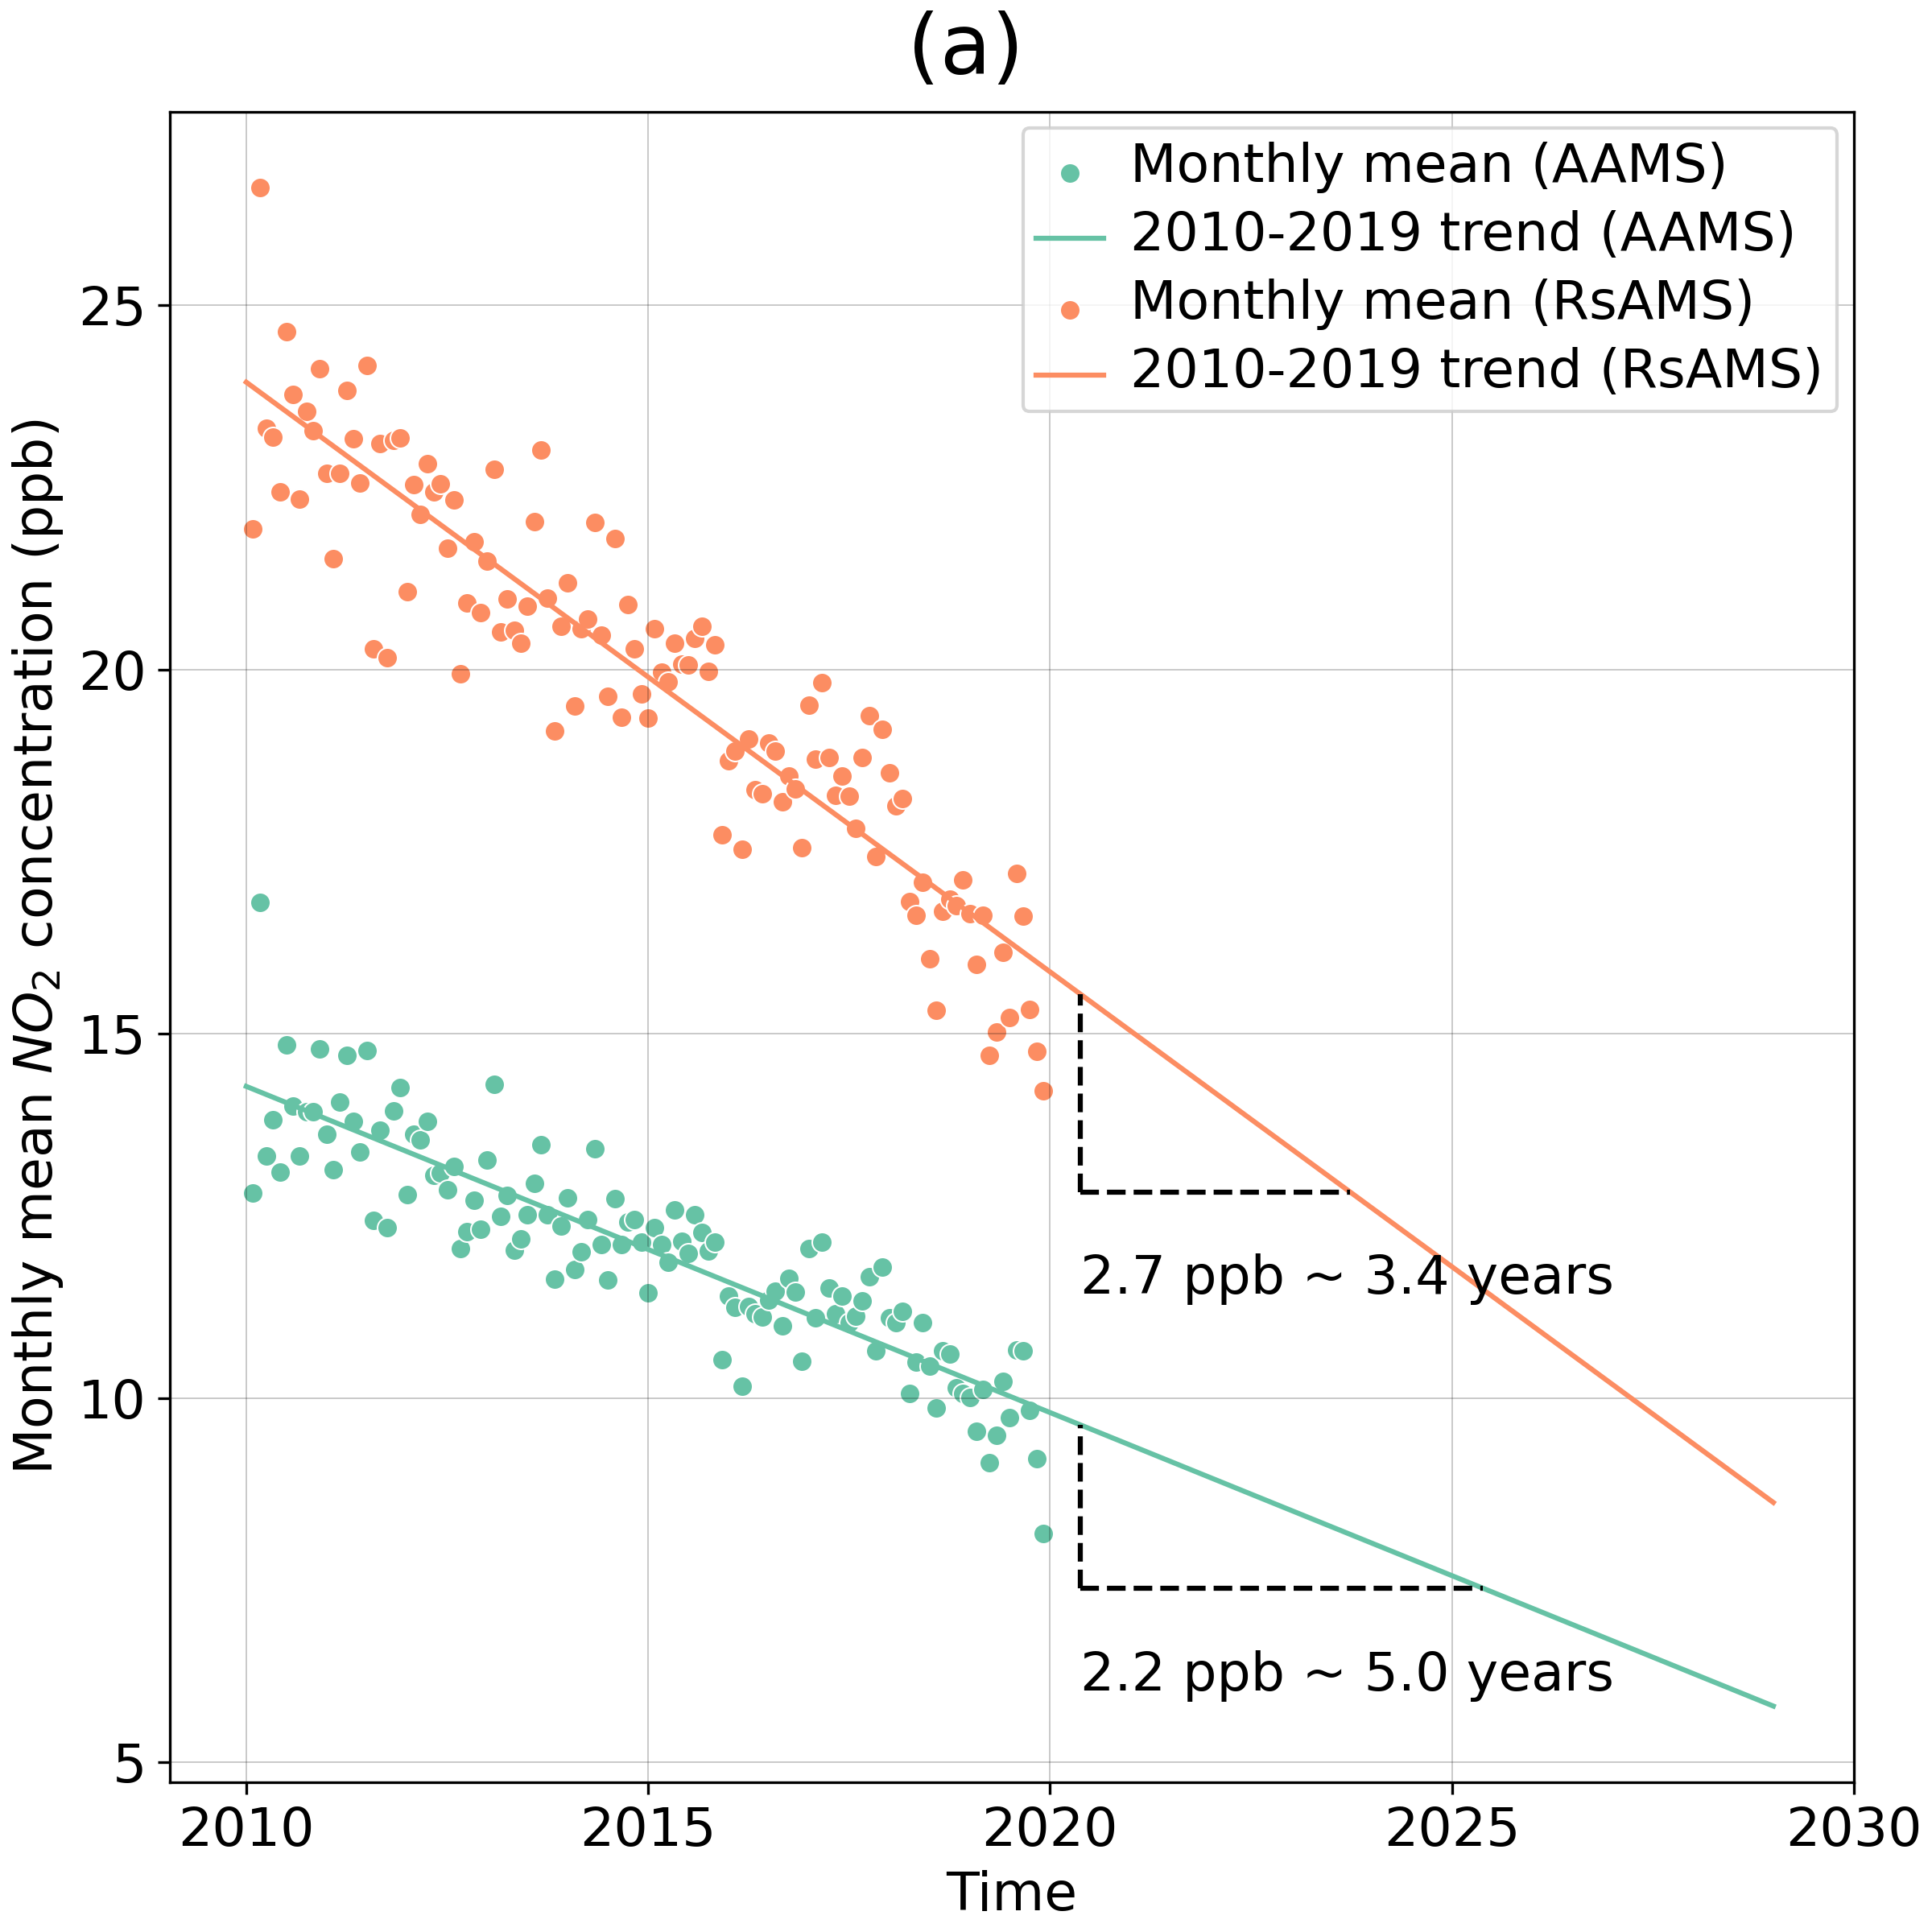
\includegraphics[width=\textwidth]{figs/chap4/fig4a.png}
      \label{fig:chap4_fig4a}
    \end{subfigure}%
    \begin{subfigure}{.5\textwidth}
      \centering
      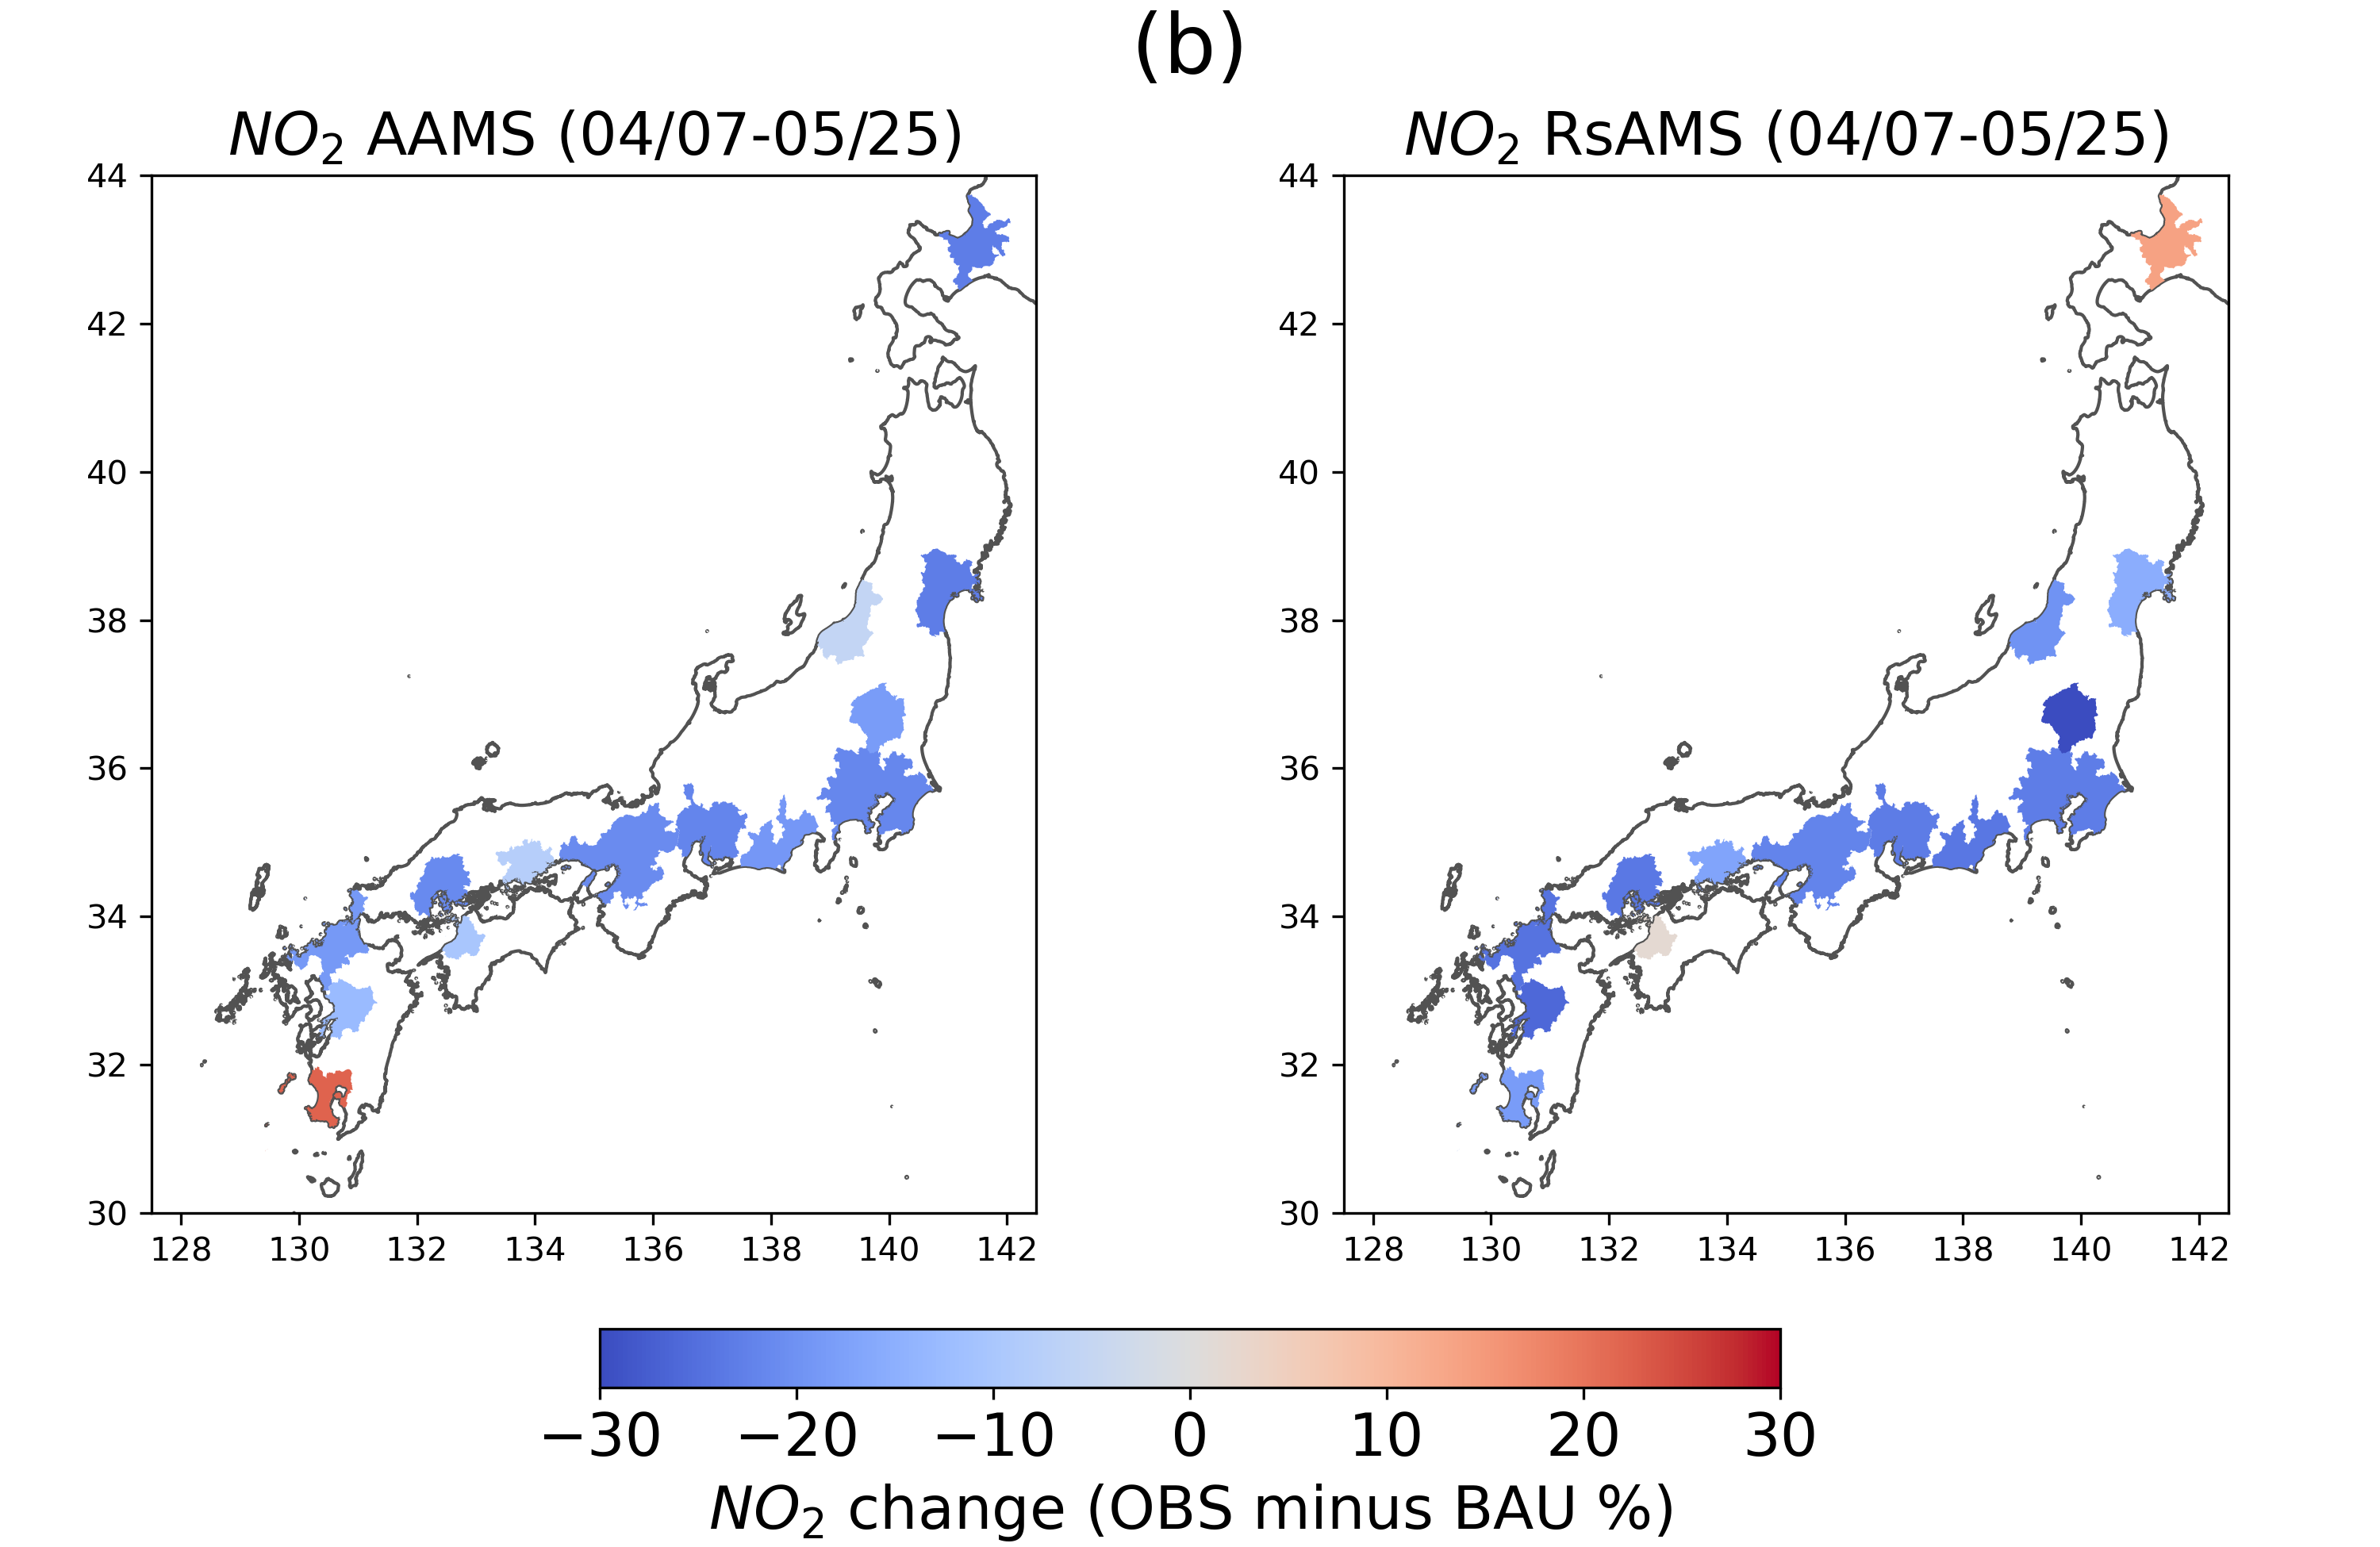
\includegraphics[width=\textwidth]{figs/chap4/fig4b.png}
      \label{fig:chap4_fig4b}
    \end{subfigure}

    \begin{subfigure}{\textwidth}
        \centering
        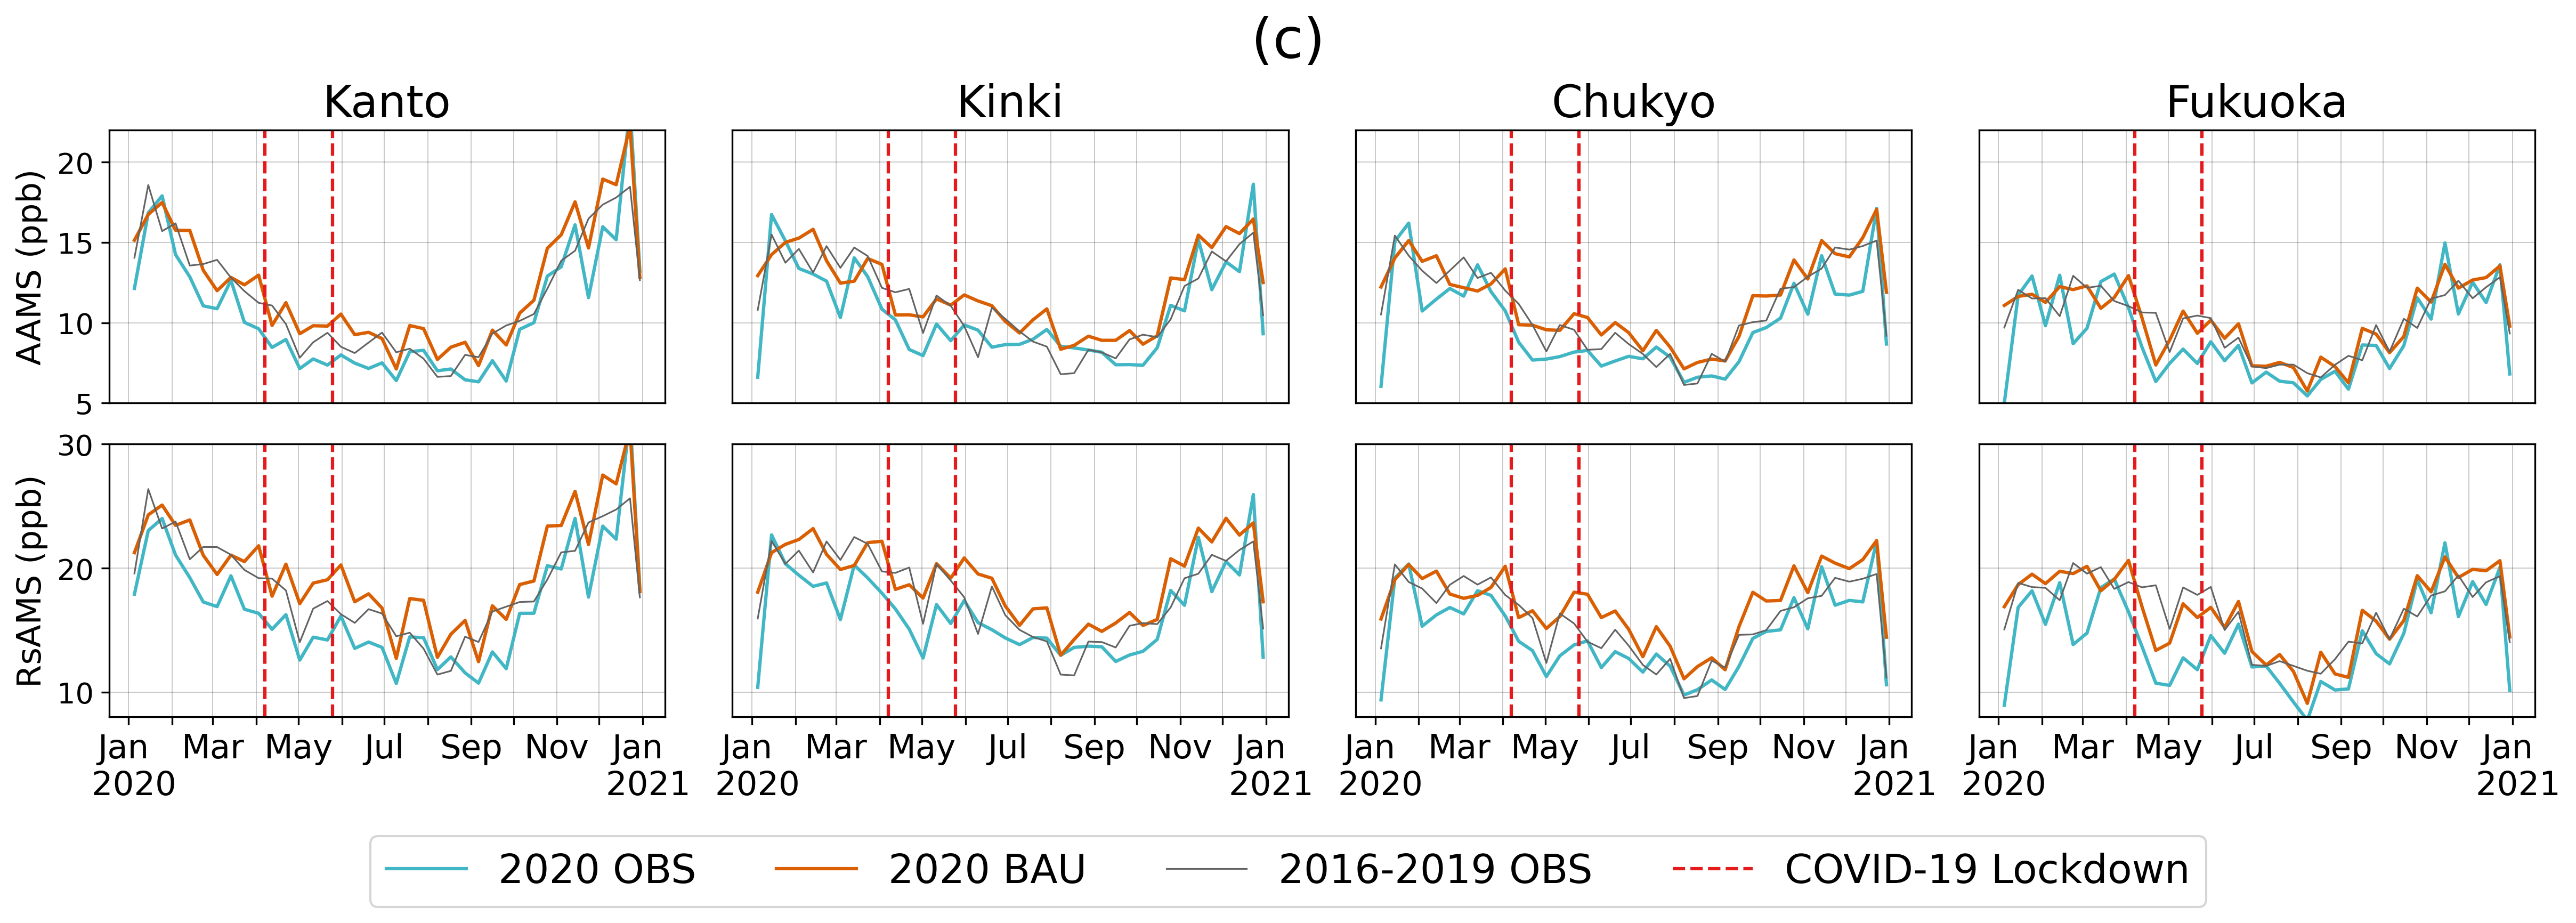
\includegraphics[width=\textwidth]{figs/chap4/fig4c.png}
        \label{fig:chap4_fig4c}
    \end{subfigure}
    \caption[NO2 reduction trends in 2020]{(a) Mean ground observation trend with the reduction in NO2 due to the lockdown in 2020 for AAMS and RsAMS. (b) Map visualization of the “OBS-BAU” estimate for NO2 during the lockdown period. (c) The 7-day rolling mean of 2020 observation (OBS), BAU prediction (BAU), and mean level of NO2 from 2016 to 2019 for 4 MAs}
    \label{fig:chap4_fig4}
\end{figure}


\begin{table}[tbh!]
    \centering
    \caption[short]{OBS-BAU estimates for NO2 during the lockdown (April 7 to May 25) and post-lockdown (August 1 to 31). For timeseries estimate, we considered all days of the week. However, when considering weekday, we only included Monday to Friday, while for weekends, we only accounted for Sunday and Saturday. The values are represented as mean (standard deviation)}
    \begin{adjustbox}{width=\textwidth}
        \begin{tabular}{c c c c c c c}
        \hline
            \multirow{3}{*}{Station type} & \multicolumn{3}{c}{Lockdown (April 7 \textminus May 25)} & \multicolumn{3}{c}{Post-lockdown (August 1\textminus31)}\\ \cline{2-7}
                & Timeseries  & Weekday  & Weekend  & Timeseries  & Weekday  & Weekend  \\
                & (\%)  & (\%)  & (\%)  & (\%)  & (\%)  & (\%)  \\ \hline
            AAMS & -14.5 (12.1) & -12.9 (14.3) & -18.4 (8.6) & -10.2 (7.3) & -6.8 (7.8) & -17.2 (8.3)  \\
            RsAMS & -19.1 (13.5) & -18.0 (14.2) & -21.9 (13.9) & -18.1 (11.2) & -13.6 (12.3) & -27.4 (10.0)  \\ \hline
        \end{tabular}
    \end{adjustbox}
    \label{tab:chap4_tab21}
\end{table}

Overall, NO2 levels exhibited a decline across most MAs. The decline in emissions was particularly significant in RsAMS compared to AAMS in most MAs, with an average reduction of 19.1\% and 14.5\% respectively. However, these reductions were smaller compared to those observed in European cities \citep{barre2021estimating,grange2021covid}. Additionally, we observed that the reduction in NO2 levels during weekends was more significant than on weekdays, primarily due to a substantial decrease in mobility during weekends compared to weekdays (refer to Figure 1b). During the lockdown the average reduction in NO2 levels for AAMS was 12.9\% on weekdays and 18.4\% on weekends. As for RsAMS, the average reduction stood at 18\% on weekdays and 21.9\% on weekends. For most MAs, even the lockdown has been lifted in the end of May 2020, the NO2 level still continue to decline until the end of December 2020. This ongoing decrease may be attributed to the sustained reduction in mobility trends from the period of the lockdown through the end of 2020 (as illustrated in Figure 1a). These findings are summarized in Table 2 and Table 3. \par

\subsection{O3 level changes}
In this experiment, we investigated various parameters to gain a better understanding of the changes in O3 in response to the reduction of NO2 caused by COVID-19 social distancing policies. Alongside the "OBS-BAU" estimates, we examined standardized anomalies of T2M and SR between 2020 and 2016-2019 period, S5P FNR in 2020, and changes in S5P HCHO between 2020 and 2019. These parameters were analyzed for two distinct periods: the lockdown period and the post-lockdown (August 1 \textminus 31), 2020. \par

\subsubsection*{Changes during the lockdown period}
During the lockdown period (April 7 to May 25), we observed a slight change in O3 levels across most MAs (Figure 5 second row and Figure 6). On average, there was a reduction of 2.3\% in AAMS and 0.6\% in RsAMS, as indicated in Table 2. Although the overall trend showed a decrease, we did find instances of increased O3 levels in certain MAs, particularly in RsAMS such as Kanto (1.6\%), Kinki (2.2 \%), and Fukuoka (3.5 \%), as depicted in Figure 5 (second row). Moreover, we have observed the existence of an "ozone weekend effect" in the changes of O3 levels, indicating higher increase in O3 mixing ratios during weekends in comparison to weekdays (Akimoto and Tanimoto 2022). This effect was observed in the "OBS-BAU" estimates for RsAMS in Fukuoka (increased 8.8\% - weekends, 1.3\% - weekdays) and Kinki (increased 4.9\% - weekends, 1.2\% - weekdays).
The observed slight decrease in O3 levels across most MAs in Japan contrasts with the trends observed in many other major cities worldwide \citep{shi2021abrupt,grange2021covid}, where significant increases in O3 levels have been observed. For instance, after accounting for weather effects, notable increases have been reported in Beijing (28.9 \%), Wuhan (44.5 \%), Milan (66.8 \%) Rome (55.8 \%), New York (17.4 \%), Los Angeles (14.8 \%), and Delhi (26.2 \%) by \citep{shi2021abrupt}.\par
To explore this variation further, we analyzed the disparity in T2M and SR between the corresponding period of 2020 and the reference period 2016-2019 as shown in Figure 5 (3rd row). We observed small positive SR anomalies in the southeast region of Japan and negative SR anomalies in the northeast region. Additionally, across the entire country, negative T2M anomalies were observed. The presence of negative T2M anomalies and fluctuating SR levels suggests that the prevailing weather conditions during this period impeded the production of O3. \par

\begin{figure}[p]
    \centering
    \includegraphics[width=\textwidth]{figs/chap4/fig5.png}
    \caption[NO2, O3, SR, T2M, FNR, and HCHO variations in 2020]{The 1st and 3rd columns show the plots for the lockdown (April 7 to May 25). The 2nd and last columns show the plots for August 1 \textminus 31. The 1st row: The OBS-BAU estimates of NO2 for AAMS and RsAMS. The 2nd row: The OBS-BAU estimates of O3 for AAMS and RsAMS. The 3rd row: The standardised anomalies of downward solar radiation (SR) and temperature (T2M) from ERA5 dataset. The last row: The formandehyle-to-NO2 (FNR) ratio in 2020 and the HCHO change between 2020 and 2019 from Sentinel 5P data.}
    \label{fig:chap4_fig5}
\end{figure}

\begin{figure}[tbh!]
    \centering
    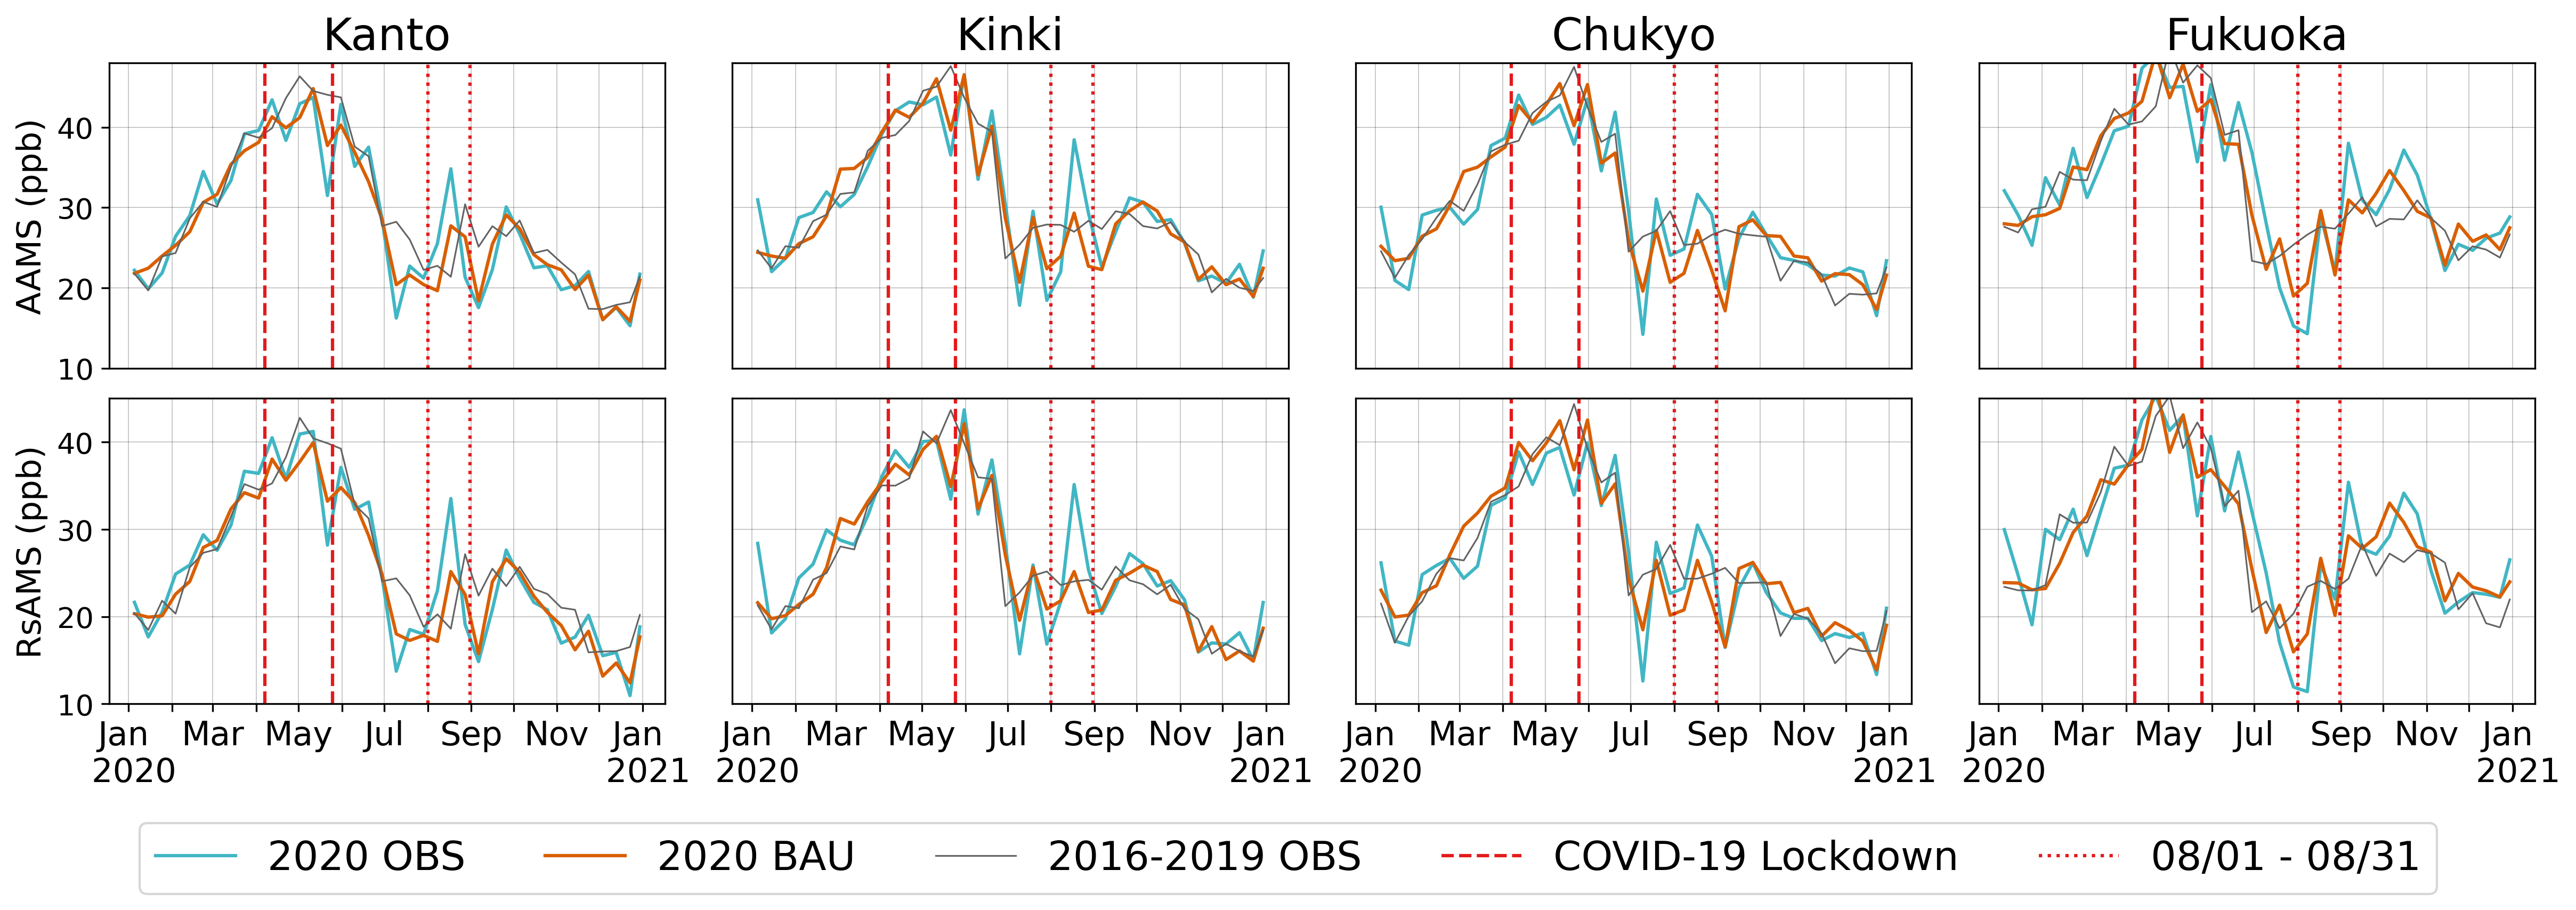
\includegraphics[width=\textwidth]{figs/chap4/fig6.png}
    \caption[2020 O3 mean trends (4 MAs)]{The 7-day rolling mean of 2020 observation (OBS), BAU prediction (BAU), and mean level of O3 from 2016 to 2019 for 4 MAs (Kanto, Kinki, Chukyo, and Fukuoka)}
    \label{fig:chap4_fig6}
\end{figure}

\begin{table}[tbh!]
    \centering
    \caption[short]{OBS-BAU estimates for O3 during the lockdown (April 7 to May 25) and post-lockdown (August 1 to 31). For timeseries estimate, we considered all days of the week. However, when considering weekday, we only included Monday to Friday, while for weekends, we only accounted for Sunday and Saturday. The values are represented as mean (standard deviation)}
    \begin{adjustbox}{width=\textwidth}
        \begin{tabular}{c c c c c c c}
        \hline
            \multirow{3}{*}{Station type} & \multicolumn{3}{c}{Lockdown (April 7 \textminus May 25)} & \multicolumn{3}{c}{Post-lockdown (August 1\textminus31)}\\ \cline{2-7}
                & Timeseries  & Weekday  & Weekend  & Timeseries  & Weekday  & Weekend  \\
                & (\%)  & (\%)  & (\%)  & (\%)  & (\%)  & (\%)  \\ \hline
            AAMS & -2.3 (2.7) & -2.7 (3.2) & -1.2 (2.7) & 2.2 (15.6) & 3.2 (15.3) & 0.0 (18.8)  \\
            RsAMS & -0.6 (2.7) & -1.4 (2.7) & 1.4 (3.7) & 8.9 (10.7) & 8.9 (12.3) & 8.6 (12.7)  \\ \hline
        \end{tabular}
    \end{adjustbox}
    \label{tab:chap4_tab22}
\end{table}

\subsubsection*{Changes during the August, 2020}
In August 2020, the NO2 levels continued to decline in all MAs, albeit at a slower rate compared to the lockdown period, as shown in Table 2. However, during this period, we observed a more noticeable increase in O3 levels across most MAs compared to the lockdown. On average, there was a 8.9\% increase for RsAMS and a 2.2\% increase for AAMS. Notably, the increase in O3 levels during weekends was more significant than on weekdays in Niigata, Okayama, Kinki and Sendai. Specifically, For AAMS of Niigata, O3 levels experienced a 9.4\% increase on weekends and a 5.8\% increase on weekdays. In RsAMS of Okayama, O3 levels saw a 13\% increase on weekends, exceeding the 10.6\% increase observed on weekdays. Similarly, in AAMS in the Kinki region, O3 levels exhibited a weekend increase of 19.8\%, surpassing the 17.4\% increase observed on weekdays. In Sendai, the increase during weekends was even more pronounced, with a 15.6\% increase for AAMS and a 22\% increase for RsAMS, whereas on weekdays the increase was 5.1\% for AAMS and 9.8\% for RsAMS. This observation could be attributed to the greater reduction in movement during weekends compared to weekdays in these MAs as show in Figure 1b. \par
In order to investigate the differences in O3 levels between August and the lockdown period, we examined the standard anomalies of SR and T2M in August 2020, comparing them to the 2016-2019 period. Our analysis revealed positive anomalies in both SR and T2M across all MAs, as shown in Figure 5 (3rd row). These favorable weather conditions, combined with the reduced levels of NO2, likely facilitated increased O3 production. \par

Although there was an overall trend of increasing O3 levels during this period, we did observe a reduction in O3 levels in five MAs which is located in the southern region: Hiroshima (AAMS: 13.7\%), Matsuyama (AAMS: 1\%, RsAMS: 3\%), Fukuoka (AAMS: 12.5\%, RsAMS: 12.3\%), Kumamoto (AAMS: 20.7\%), and Kagoshima (AAMS: 29.9\%). To understand the decrease in O3 levels observed in these five MAs, we utilized the S5P FNR for 2020, as well as the changes in HCHO as a proxy for NMVOCs between 2020 and 2019. The FNR is commonly used to assess the sensitivity of near-surface O3 levels \citep{martin2004space}. As suggested by \citep{duncan2010application}, when the FNR is below 1, the O3 production regime is considered VOC-limited, and when it exceeds 2, it is considered NOx-limited. When the FNR values fall within the range of 1\textminus2, O3 is expected to be in the transition regime \citep{duncan2010application}. However, it has been observed that the FNR can vary by region \citep{jin2020inferring,irie2021continuous,souri2023characterization,ren2022diagnosing}, and the assumption that it lies within the 1\textminus2 range may not hold true at the global level \citep{schroeder2017new}. Hence, it might be essential to calculate this ratio on a regional scale \citep{damiani2022peculiar,schroeder2017new}. Despite the FNR showing high variability in the region, it still provides information about the trend of O3 production regimes in our study. \par
Figure 5 (last row) presents the FNR across all MAs indicating a shift in the O3 production regime from VOC-limited during the initial lockdown to NOx-limited in August. This transition is evident as the FNR changes from 0 < FNR < 2 during the lockdown to FNR > 4 in August. During the VOC-limited regime, a decrease in NOx typically leads to an increase in O3 levels \citep{duncan2010application}. However, in the NOx-limited regime, a reduction in NOx can also result in a decrease in O3 levels \citep{duncan2010application}. In Figure 5 (last row), we can observe that the NOx-limited regime dominates the five MAs of Hiroshima, Matsuyama, Fukuoka, Kumamoto, and Kagoshima. Despite NO2 levels continuing to decline during this period, the HCHO levels exhibited a more significant increase in these MAs compared to the lockdown period. Hence, this could explain the reduction in O3 levels observed in these five southern MAs. \par
We elucidated the difference in O3 levels between major MAs in Japan and other large urban areas worldwide by examining meteorological changes (T2M, SR), and variations in O3 precusors levels by utilizing S5P FNR derived from S5P NO2 and HCHO measurements. The difference can be attributed to the absence of sunny conditions during the lockdown period. However, in August, when sunny conditions became more prevalent, we observed an increase in O3 levels in response to the sustained reduction in NO2 levels across most MAs, which are likely VOC-limited areas. Based on the analysis of S5P data, it appears that the southern metropolitan areas (MAs) exhibited a predominant NOx-limited trend during August 2020, potentially due to the increased presence of biogenic VOCs (BVOCs). However, the monitoring of BVOCs emissions remains challenging due to limited observations \citep{tani2021exchanges,ito2021terrestrial}. Therefore, it is also important to pay attention to those NOx-limited areas, as future reductions in anthropogenic NMVOCs may have minimal effectiveness in reducing O3 levels (Akimoto and Tanimoto 2022). \par

\subsection{CH4 level changes}
In this experiment, we analyze the "OBS-BAU" estimates for NO2, CO, and CH4, and incorporate the VISIT model's simulated CH4 emissions from wetlands to investigate the changes in CH4 levels during the 2020 lockdown and post-lockdown period. Our focus is on understanding the relationship between the reduction in NO2 and its potential impact on OH (hydroxyl radicals), as well as the contrasting effect of CO. The decrease in NO2 levels is expected to result in a reduction in OH, while reductions in CO can increase OH levels and shorten the lifetime of CH4 \citep{akimoto2022rethinking}.\par
During the lockdown period, we observed a marginal rise in CH4 levels across most MAs (Figure 7 third row and Figure 8b), with an average increase of 0.6\% for AAMS and 0.8\% for RsAMS (Table 3). While NO2 levels decreased in most MAs (Figure 7 first row), the trend for CO varied (Figure 7 second row and Figure 8a). AAMS showed an average decrease of 10.9\% in CO levels, while RsAMS saw a slightly smaller reduction 8.8\%. Notably, CO levels significantly increased in RsAMS of Kagoshima (60.6\%), while slight increases were observed in Kanto AAMS, and in Matsuyama for both RsAMS and AAMS. It is worth noting that although the increases in CO levels in Kagoshima were significant, this region have among the lowest natural CH4 emissions in Japan as Figure 7 (last row), which explains the slight increase in CH4 observed in this MA.\par


\begin{figure}[p]
    \centering
    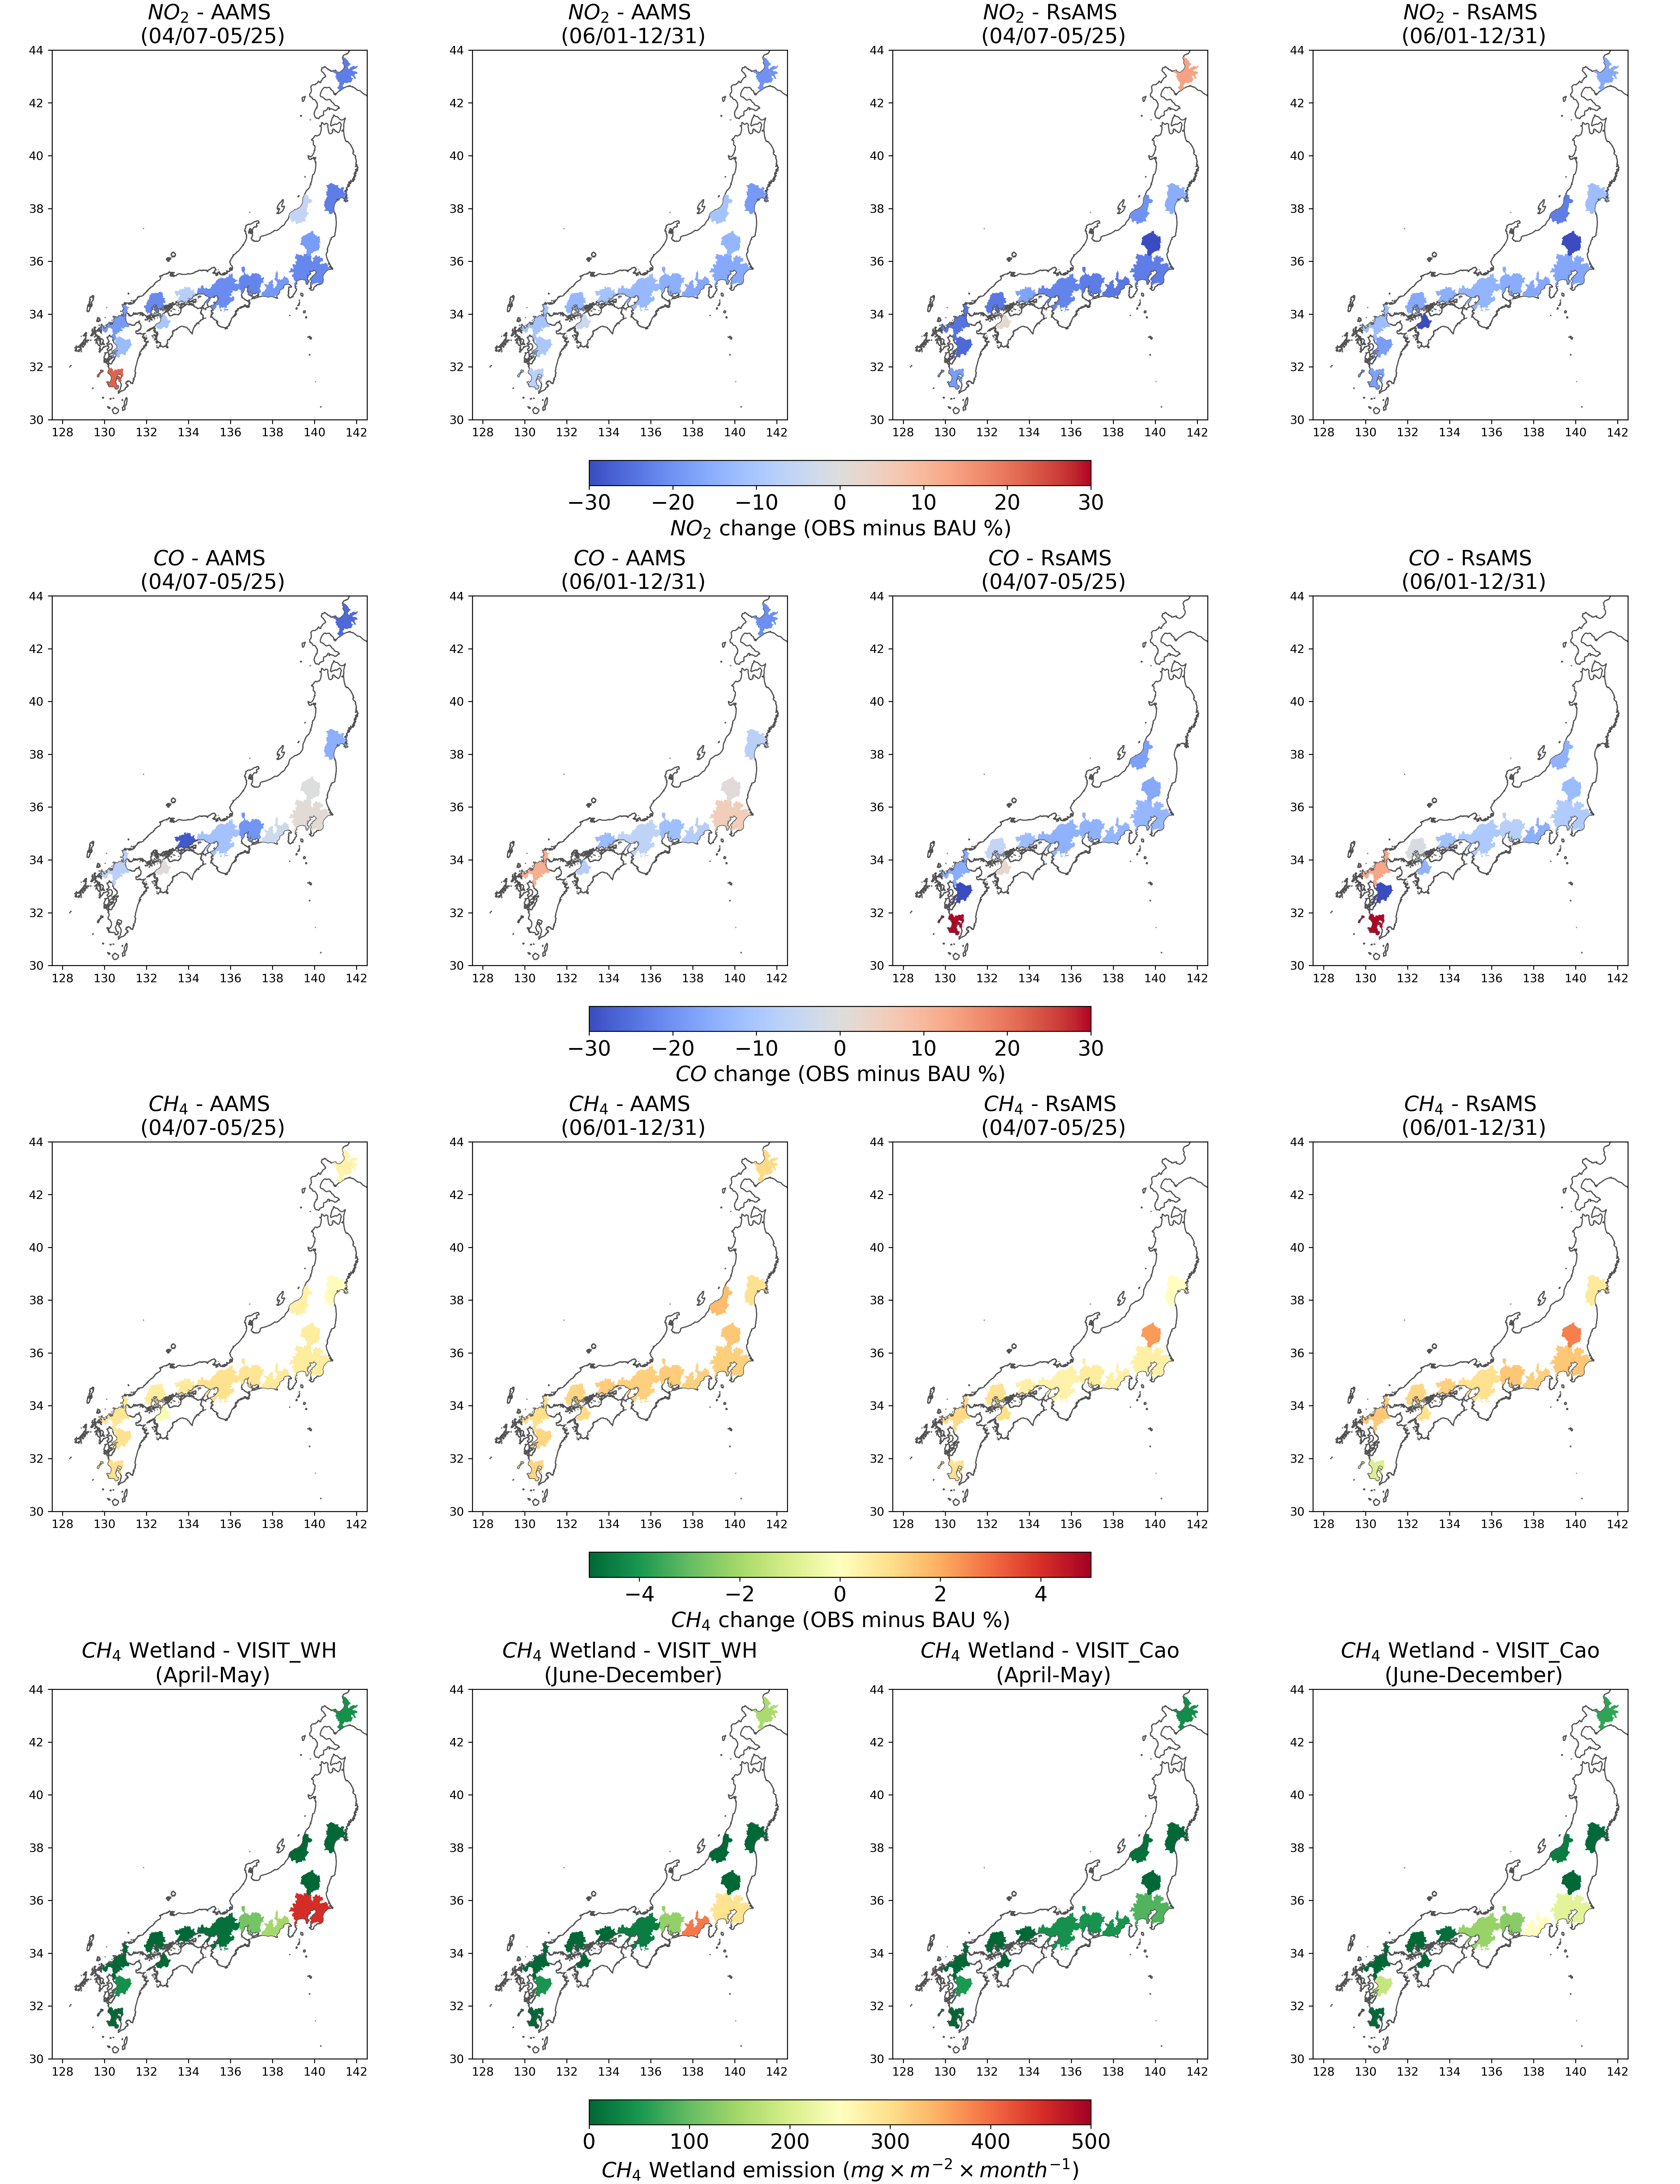
\includegraphics[width=\textwidth]{figs/chap4/fig7.png}
    \caption[NO2, CO and CH4, and HCHO variations in 2020]{The 1st and 3rd columns show the plots for the lockdown (April to May). The 2nd and last columns show the plots for the post-lockdown (June to December). The 1st row: The “OBS-BAU” estimates of NO2 for AAMS and RsAMS. The 2nd row: The “OBS-BAU” estimates of CO for AAMS and RsAMS. The 3rd row: The “OBS-BAU” estimate of CH4 for AAMS and RsAMS. The last row: The CH4 emission from wetland based on the simulation of VISIT model with Walter and Heimann scheme and Cao scheme.}
    \label{fig:chap4_fig7}
\end{figure}


\begin{figure}[tbh!]
    \centering
    \begin{subfigure}{\textwidth}
      \centering
      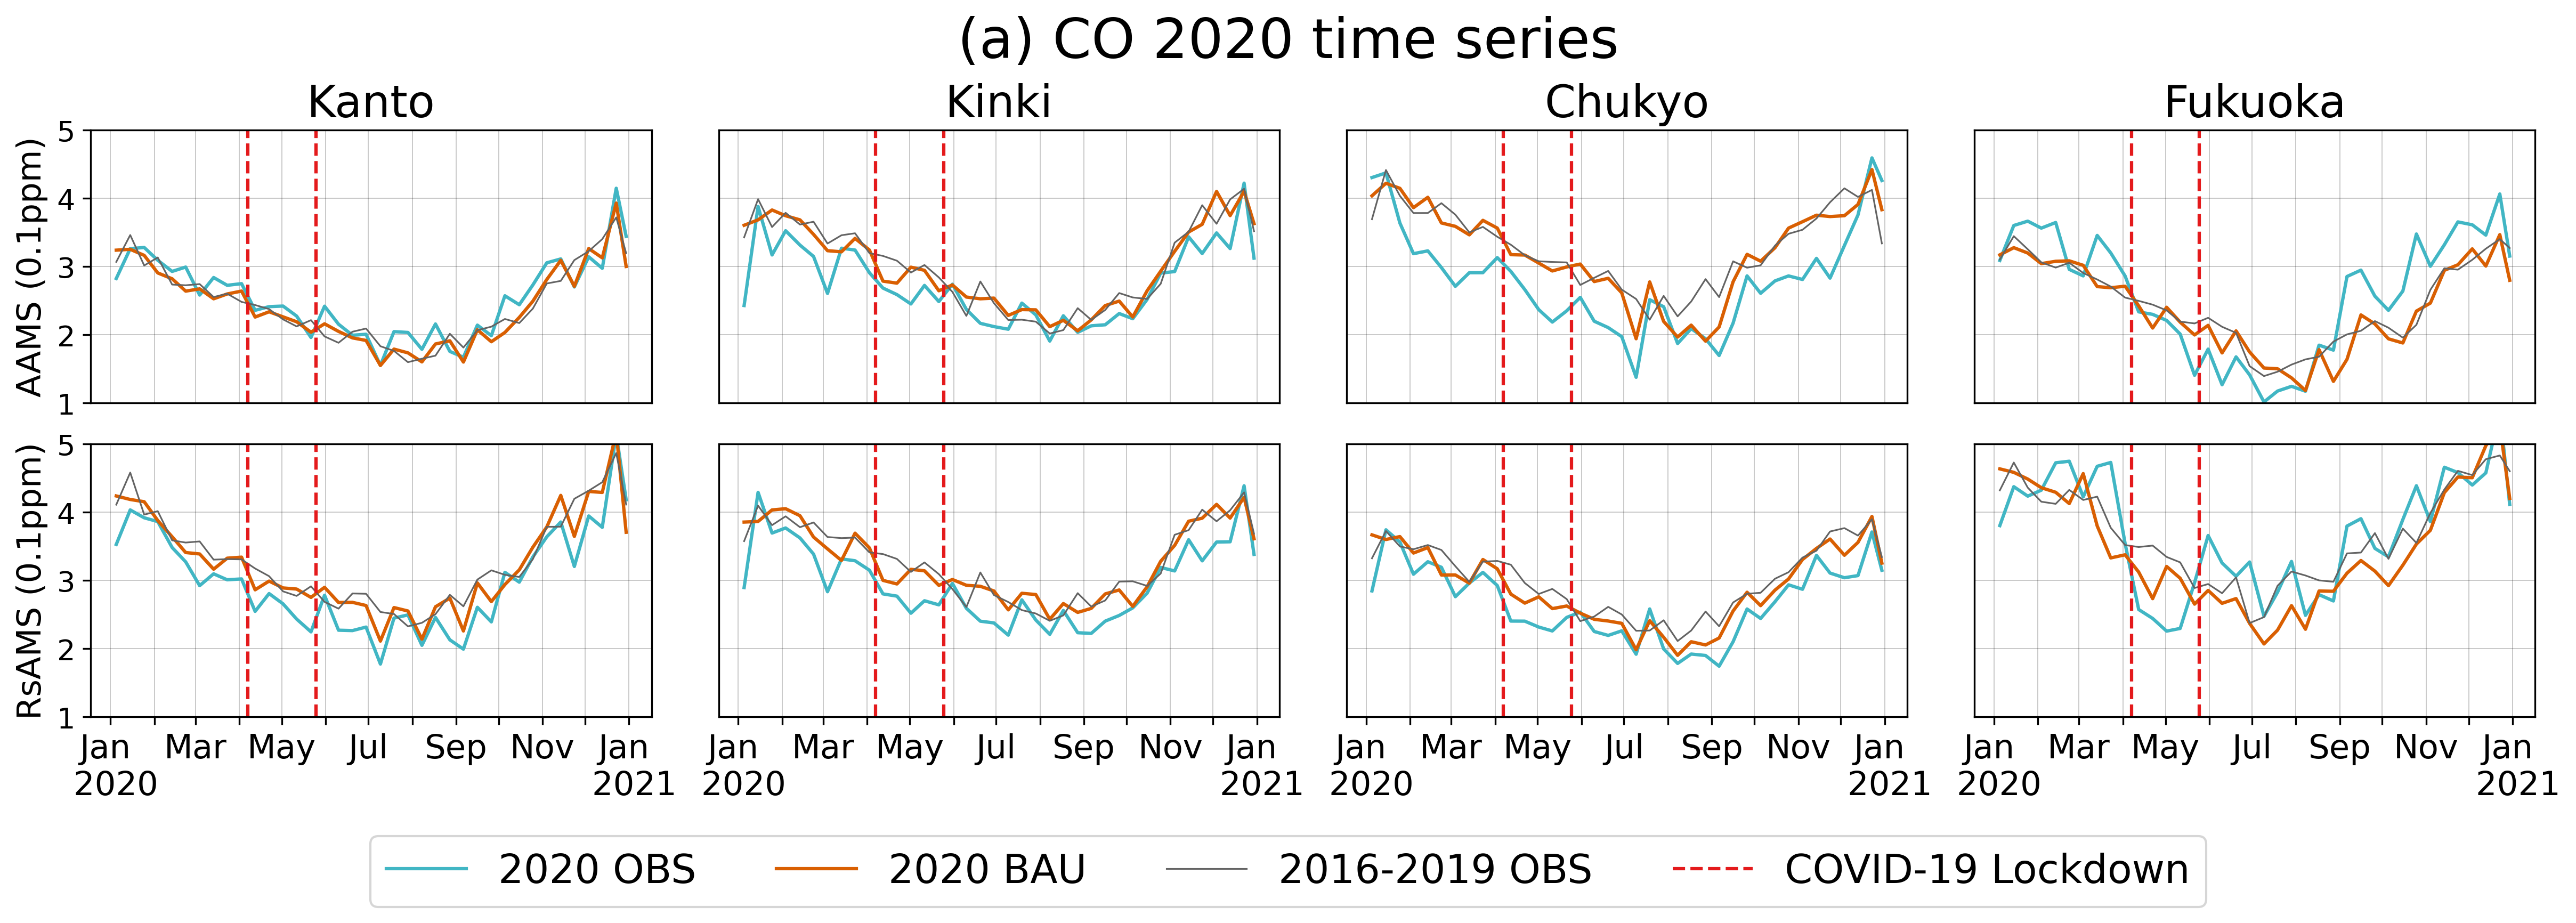
\includegraphics[width=\textwidth]{figs/chap4/fig8a.png}
      \label{fig:chap4_fig8a}
    \end{subfigure}

    \begin{subfigure}{\textwidth}
      \centering
      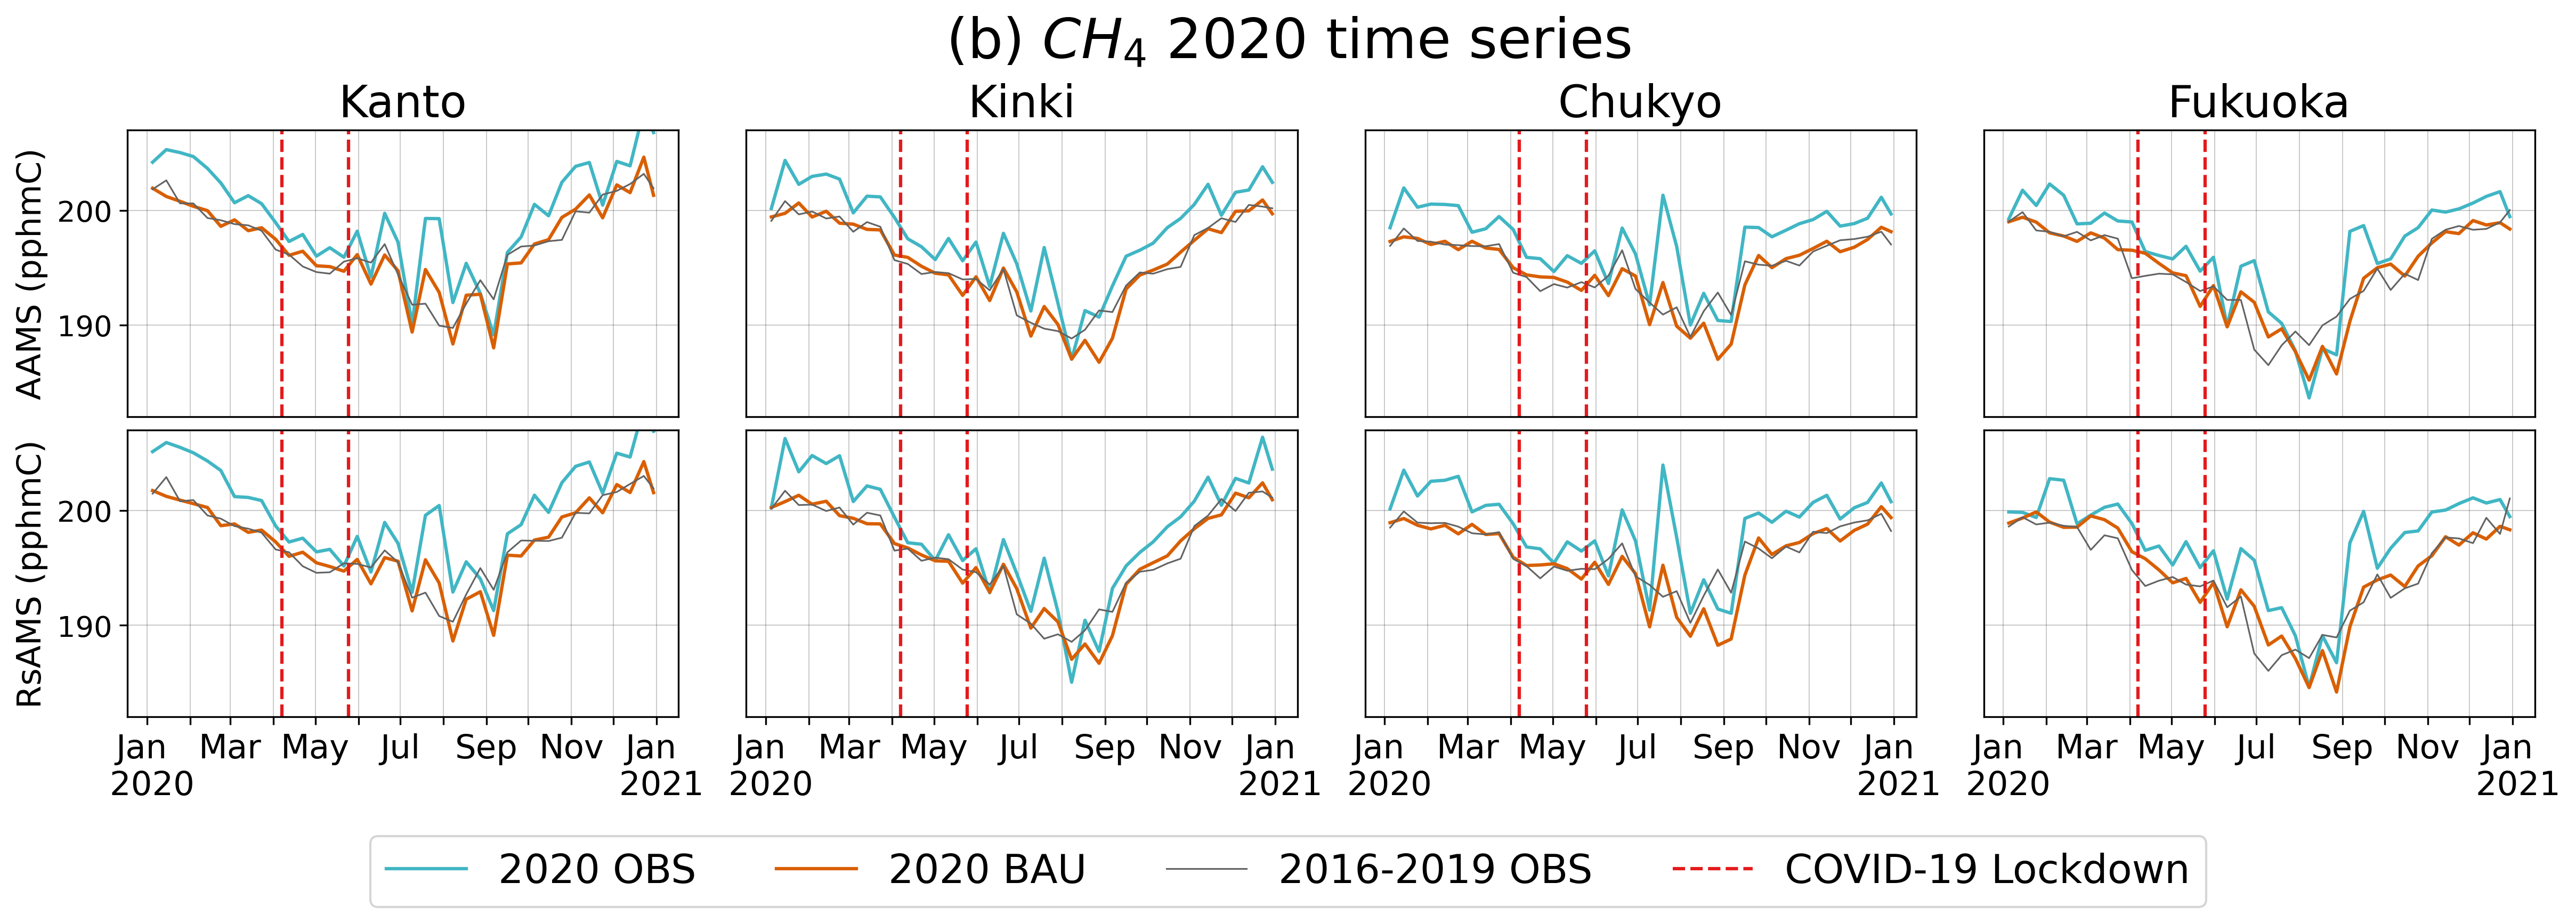
\includegraphics[width=\textwidth]{figs/chap4/fig8b.png}
      \label{fig:chap4_fig8b}
    \end{subfigure}
    \caption[2020 CO and CH4 mean trends (4 MAs)]{The 7-day rolling mean of 2020 observation (OBS), BAU prediction (BAU), and mean level of CO (a) and CH4 (b) from 2016 to 2019 for 4 MAs (Kanto, Kinki, Chukyo, and Fukuoka)}
    \label{fig:chap4_fig8}
\end{figure}

\begin{table}[tbh!]
    \centering
    \caption[short]{OBS-BAU estimates for NO2 and CO and CH4 during the lockdown (April 7 to May 25) and the post-lockdown (June 1 to December 31). For CH4 analysis we only consider timeseries estimate which include all days of the week. The values are represented as mean (standard deviation)}
    \begin{tabular}{c c c c}
    \hline
    \multirow{2}{*}{Pollutant} & \multirow{2}{*}{Station type} & (April 7 – May 25) & (June 1 – December 31) \\ 
                                &                              & (\%) & (\%) \\ \hline
    \multirow{2}{*}{NO2} & AAMS & -14.5 (12.1) & -12.8 (4.3)  \\
        & RsAMS & -19.1 (13.5) & -18.3 (6.4)  \\ \hline
    \multirow{2}{*}{CO} & AAMS & -10.9 (11.0) & -5.7 (9.4)  \\
        & RsAMS & -8.8 (24.6) & -5.5 (25.2)  \\ \hline
    \multirow{2}{*}{CH4} & AAMS & 0.6 (0.3) & 1.3 (0.2)  \\
        & RsAMS & 0.8 (0.6) & 1.1 (0.9)  \\ \hline
    \end{tabular}
    \label{tab:chap4_tab3}
\end{table}

During the post-lockdown period from June to December 2020, NO2 levels continued to decrease, showing an average reduction of 12.8\% for AAMS and 18.3\% for RsAMS (Table 3) which is smaller than during the lockdown period. In contrast, CO levels started to recover as the COVID-19 lockdown was lifted, with a smaller reduction of 5.7\% for AAMS and 5.5\% for RsAMS. Notably, significant increases in CO levels were still evident at RsAMS in Kagoshima (62.2\%). In Fukuoka we also observed a steady rise of CO levels in both RsAMS (13\%) and AAMS (11.5\%). In response to these changes in NO2 and CO, we observed a greater increase in CH4 levels during this period, with a rise of 1.3\% for AAMS and 1.1\% for RsAMS.\par
In general, we saw a slight increase in CH4 levels both during the lockdown and the post-lockdown periods, based on the "OBS-BAU" estimates. However, a more pronounced increase in CH4 was observed during the post-lockdown phase in AAMS when compared to RsAMS, which can be attributed to the more substantial recovery of CO levels in AAMS relative to the lockdown period. Although it has been reported that global CH4 growth in 2020 is primarily attributed to the atmospheric sink resulting from lower anthropogenic NOx emissions \citep{stevenson2022covid,peng2022wetland}, our findings regarding the contribution of NOx reduction to the CH4 growth in Japan in 2020 align with a previous study \citep{akimoto2022rethinking,qu2022attribution,feng2023methane}, indicating that the impact of NOx and CO change on the increase in CH4 growth in Japan during the lockdown and post-lockdown period is not as significant as the direct CH4 emission itself. \par

\section{Discussion} \label{chap4_disscussion}
\subsection{Variations in spatial resolution of multisource data}
Since we utilized multisource data for the analysis, we acknowledge that variations in spatial resolution among input data can influence the consistency and reliability of data analysis. In certain situations, the need for interpolation to achieve a uniform grid may arise, particularly when generating inputs for a Convolutional Neural Network (CNN). This interpolation process inadvertently introduces uncertainty into the results.  However, in this study, we refrained from any data interpolation and used it at its provided original resolution. The multisource data was employed for two primary objectives: weather-normalization model development and visual examination purpose. \par
For weather-normalization model development, we used ERA5 data and ground station data to construct the weather-normalization model. Certain variables, such as total cloud cover and boundary layer height, are exclusively available from ERA5. The ERA5 data we employed has a resolution of 0.25° × 0.25°, meaning that some stations might share identical ERA5 records. This can influence the model development, even though, ideally, local ERA5 values for each station should be distinct, albeit not significantly deviating from the 0.25° × 0.25° spatial resolution value. To mitigate this effect on the model development, we have integrated spatial context values (latitude and longitude) and station types as additional inputs. Since these features are distinct for each station, we anticipate that they can help minimize the impact of the coarse spatial resolution from ERA5 on the model. \par
To visually inspect the sensitivity of tropospheric O3 production utilizing S5P HCHO and NO2, as well as CH4 emission estimates from wetland, we rely exclusively on original data with consistent spatial resolution. It's important to note that our primary focus is to visually inspect the prevailing trends at the MA level, which has a spatial resolution coarser than that of any input data we utilized. Therefore, we believe that the dominant trends at the MA level remain unaffected by these spatial disparities in this particular MA-level context. \par

\subsection{Limitations}
In this research, we utilized the S5P FNR to examine the sensitivity of O3 production. Although HCHO could be an alternative indicator for NMVOCs presence, the significant uncertainty in the FNR threshold from previous studies, along with the lack of NMVOCs observations and reliable satellite HCHO and NO2 data, poses challenges in understanding O3 level variations during and after the lockdown period. This issue is particularly crucial and warrants in-depth exploration in future studies. \par
Additionally, it's important to mention that the study did not include an analysis of long-range air pollution transportation from China to western MAs of Japan following the Chinese economic recovery from the pandemic \citep{itahashi2022returning}. This aspect was beyond the scope of the current research but should be considered in future investigations. \par

\section{Conclusion} \label{chap4_conclusion}
This study presents an air quality analysis that examines the changes in four air pollutants, namely NO2, O3, CO, and CH4, during the COVID-19 pandemic in 14 MAs of Japan from April 7 to December 31 in 2020. Firstly, we developed a machine learning BAU model that incorporates meteorological, spatial, and temporal features to account for weather variability in air quality time series. Next, we utilized the BAU model predictions and observation data to estimate the actual reduction (OBS-BAU estimate) in NO2 levels. We then integrated temperature and solar radiation anomalies from ERA5 reanalysis data and S5P TROPOMI data (FNR and HCHO) along with the “OBS-BAU” estimate to investigate the unique response of O3 to the NO2 reduction during the lockdown and post-lockdown period (August 1 – 31, 2020). Finally, we evaluated the impact of NO2 and CO changes on the CH4 levels using a combination of “OBS-BAU” estimate and wetland CH4 emission simulations from the VISIT model. The main findings of the study can be summarized as follows:\par
Based on ground observations of NO2, the reduction of NO2 during the lockdown period in 2020 corresponds to a decrease equivalent to 3.4 years and 5 years of the 2010-2019 trend of NO2 for roadside and ambient air monitoring stations respectively. After normalizing the meteorological effects by BAU predictions, the NO2 reduction was 14.5\% for AAMS and 19.1\% for RsAMS. The decrease in NO¬2 levels is more pronounced during the weekend than on weekdays.\par
By analyzing ground observations of NO2 and O3, along with BAU simulations and meteorological data from ERA5, as well as FNR and HCHO data from S5P TROPOMI, we found that the reduction in NO2 levels during the lockdown did not immediately result in an increase in O3. Instead, we observed that the increase in O3 occurred after the lockdown, specifically in August when sunny conditions were reinforced. This finding is significant for Japan, as it has not been previously reported in other studies.\par
Furthermore, when analyzing the ground observations of NO2, CO, and CH4 alongside BAU simulations and model-simulated CH4 emissions from wetlands, we found that the changes in NO2 and CO contributed marginally to the variations in CH4 levels, ranging from 0.6\% to 1.3\%, across the study areas. This finding aligns with previous studies \citep{akimoto2022rethinking,qu2022attribution,feng2023methane}, but also differs from others where the reduction in atmospheric sink has been reported as a major contributor to increased CH4 levels \citep{stevenson2022covid,peng2022wetland}.\par
Based on the findings of this study, we recommend simultaneous reduction of air pollutants and anthropogenic VOCs as well as biogenic VOCs to mitigate the adverse effects on O3 and CH4. These pollutants are significant SLCPs that can have detrimental impacts on future climate mitigation efforts. Therefore, it is crucial to address both air pollutants and VOCs emissions to effectively mitigate these adverse effects in the future policies. \par
